\chapter{Analytic model of nondegenerate internal squeezing} %Research chapter: ...
\label{chp:nIS_analytics}

% results: interpret deep and far, and be very critical of assessing your approach
% present analysis of model and decisions/approximations made
% think about the story!
% systematic and diligent
% wring all of the information out of the results/figures, find the importance and the physics

% separate this into multiple .tex files once structure finalised

%%%%%%%%%%%%%%%%%%%%%%%%%%%%%%%%%%%%%%%%%%
% chapter introduction

\jam{(Fix up mentions of nondegenerate internal squeezing in background chapters, either explain it earlier or do not confuse the reader)}

% combine the all-optical approach of dIS with the mode structure of sWLC
In this chapter, I present my analytic, Hamiltonian model of nondegenerate internal squeezing and discuss its immediate results.
%Nondegenerate internal squeezing is the same configuration as degenerate internal squeezing except that the squeezer is operated nondegenerately, but it is better thought of as an all-optical alternative to stable optomechanical filtering.
Firstly, I will review the limited literature available about nondegenerate internal squeezing, and conclude that the system with optical loss has never been fully characterised. Secondly, I will present my model and derive and characterise the sensitivity of the configuration. I will partially verify the model by demonstrating that it obeys the expected low and high loss limits, and I will show that the system is stable. Finally, I will find the threshold of nondegenerate internal squeezing using an observation that unites the different squeezing configurations in this thesis. 
% from the view of quantum optics, gravitational waves in the next chapter
This chapter is directed at understanding nondegenerate internal squeezing for general quantum metrology. In the following chapters, I will return to the problem of kilohertz gravitational-wave detection and whether nondegenerate internal squeezing can feasibly improve sensitivity. 


\section{Literature review}
% a gap in the literature, should be much shorter than the review in Section~\ref{sec:literature_review} -- maybe combine it with that one?
% cannot cite personal communication?
% claim: the modelling of this configuration has never been done as thoroughly as my work, explain why (recency of interest)

\jam{(How to be thorough with this section?)}

The available literature on nondegenerate internal squeezing is limited. Although nondegenerate OPOs have long been studied for tests of the EPR-paradox~\cite{Reid1989,Schori2001} and other applications~\cite{,,}, placing a nondegenerate squeezer in a coupled cavity system \jam{has only been studied in ... (I am not aware of any other mentions than Li2020, ask the supervisors.)}. 
Although nondegenerate internal squeezing is motivated by the two configurations in the previous chapter, those configurations have only been studied in the last few years, see Section~\ref{sec:literature_review}. \jam{(Is there direct mention of nIS in the dIS literature?)}
The only direct mention of nondegenerate internal squeezing \jam{(that I could find, check this!)} in the literature is the brief suggestion in Ref.~\cite{Li2020} that it is equivalent to stable optomechanical filtering in the lossless case. In that paper and subsequent work by the same authors~\cite{Li2021}, only mechanical loss is included in the model since it is the dominant source of loss. By the modal equivalence in Section~\ref{sec:modal_equivalence}, I predict that optical loss in the idler mode should be the dominant source of loss for nondegenerate internal squeezing but this is not known. Therefore, I identify this as a gap in the literature, no work has fully characterised nondegenerate internal squeezing with optical loss in every mode, which matters because understanding how the different losses behave determines the feasibility of the design for detection.
 % distribution of loss in applications might be far from uniform, e.g.\ how the detection loss is predicted to be higher than any of the intra-cavity losses for future gravitational-wave detectors~\cite{}.
Not only are the quantum noise and signal responses of the lossy system not known, but other aspects of understanding the system, such as its limits and the squeezing threshold, are not either. I partially fill this gap in this thesis \jam{(colloquial?)}.


\section{Analytic model}

\begin{figure}
	\centering
	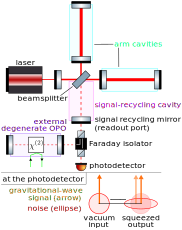
\includegraphics[width=\textwidth]{nIS_config.pdf}
	% squeezing ellipse and signal arrow plot
	\caption{\jam{(Purpose: explain configuration)} \jam{(Placeholder figure. Needs idler mode and mode labels, integrate figures on right into configuration. This is the reference for the derivation, so explain as many symbols as possible.)} Nondegenerate internal squeezing configuration with all modes and losses labelled. The idler mode is not resonant in the arms. The system's response is shown using the signal arrow and noise ellipse representation from Fig.~\ref{fig:extSqz_config}. Compare to degenerate internal squeezing in Fig.~\ref{fig:dIS_config} and the nondegenerate OPO in Fig.~\ref{fig:nOPO_config}.}
	\label{fig:nIS_config}
\end{figure}

Nondegenerate internal squeezing consists of a nondegenerate squeezer placed inside the signal-recycling cavity of an interferometer, as shown in Fig.~\ref{fig:nIS_config}. It is the same configuration as degenerate internal squeezing, shown in Fig.~\ref{fig:dIS_config}, except that the squeezer is operated nondegenerately, but it is better thought of as an all-optical alternative to stable optomechanical filtering, see Section~\ref{sec:modal_equivalence}. In the single-mode approximation, I consider the signal and idler modes resonant in the signal-recycling cavity, where the signal mode of the squeezer is at the carrier frequency $\omega_0$ and is resonant in the arms, while the idler mode at $\omega_0+\Delta$ is not resonant in the arms so that the arm and idler modes are not directly coupled, see Section~\ref{sec:modal_equivalence}. 
I model this configuration using the Hamiltonian method demonstrated several times in this thesis, and in particular, this model combines the nondegenerate OPO and degenerate internal squeezing models in Sections~\ref{sec:nOPO}~\ref{sec:dIS_model}, respectively. % There are no steps in this derivation that have not already appeared in this thesis \jam{(check this)}.
This model is based on and verified, in the lossless case, against Ref.~\cite{Li2020}. 
% \jam{(Probably need to talk about my methodology more -- state that this derivation presented is the last of a long line of increasing complexity (more losses, radiation pressure, pump phase, etc.) and that I have verified at each stage that the model recovers the previous model. This allowed me to also consider the impact of each subsequent addition in isolation. Moreover, I should re-emphasise that it reduces to the lossless case in Li and follows the same path as the verified models of dIS and the OPOs. The point is that this derivation is not controversial.)}
My methodology when constructing this model was to start with the lossless model in Ref.~\cite{Li2020} and progressively add each complication of optical loss in each mode, radiation pressure, and pump phase. At each stage of the progression, I verified that the model recovered the previous stage in the appropriate limits. This allowed me to study the effect of each complication separately rather than study the full model all at once. \jam{(need to be more critical of the approach?)} But, for brevity, I present the full model here.

Let the modes be labelled as shown in Fig.~\ref{fig:nIS_config}, which is as in Section~\ref{sec:dIS_model} but with the addition of $\hat c$ for the idler mode as in Section~\ref{sec:nOPO}. The Hamiltonian of this system is $\hat H = \hat H_0 + \hat H_I + \hat H_\gamma + \hat H_\text{GW}$ where~\cite{} \jam{(fill in Langevin Hamiltonian)}
\begin{align}
\hat H_0 &= \hbar \omega_0 \hat a^\dag \hat a + \hbar \omega_0 \hat b^\dag \hat b+ \hbar (\omega_0+\Delta) \hat c^\dag \hat c + \hbar (2\omega_0+\Delta) \hat u^\dag \hat u\\
\hat H_I &= i\hbar\omega_s(\hat a\hat b^\dag-\hat a^\dag\hat b) + \hbar \frac{x}{2} (e^{i\phi} \hat u \hat b^\dag \hat c^\dag+e^{-i\phi} \hat u^\dag \hat b \hat c) \\
\hat H_\gamma &= \int \ldots \\
\hat H_\text{GW} &= -\alpha (\hat{x}-L_\mathrm{arm}h(t))\left(\frac{\hat{a}+\hat{a}^\dag}{\sqrt{2}}\right)+\frac{1}{2\mu}\hat{p}^2.
\end{align}
As before, $\hat H_0$ describes the decoupled optical system, $\hat H_I$ describes the interaction between the three intra-cavity modes, $\hat H_\gamma$ describes the input/output coupling through the readout and loss ports listed below, and $\hat H_\text{GW}$ describes the coupling to the gravitational-wave signal and the evolution of the test mass mechanical mode.
There is vacuum entering the system intra-cavity to all three modes $\hat n^L_a, \hat n^L_b, \hat n^L_c$, at the readout port $\hat B_\text{in}, \hat C_\text{in}$, and in the detection chain $\hat n^L_\text{PD}$ which will be included later. Only the vacuum entering the readout port is present in the lossless model.
The Heisenberg-Langevin equations-of-motion for these operators can be found as before, using the bosonic and canonical commutation relations with all other commutators zero. I again (1) make the semi-classical and no-pump-depletion approximations to simplify the pump mode $\hat u\mapsto u=2\chi/x$, these approximations are valid below threshold, (2) enter the Interaction Picture to ignore $\hat H_0$, and (3) take fluctuating components of each operator but keep it implicit in the notation ($\delta\hat{Q}(t)\mapsto\hat{Q}$) because it does not change the equations-of-motion \jam{(is this true? it is not clear to me)}. I find the equations-of-motion to be
\begin{equation}\label{eq:nIS_EoM}
\begin{cases}
\dot{\hat{a}}=-\omega_s\hat{b} - \gamma_a \hat{a} + \sqrt{2\gamma_a}\hat{n}^L_a+\frac{i}{\hbar}\alpha(\hat{x}-L_\mathrm{arm}h)\frac{1}{\sqrt{2}}\\
\dot{\hat{b}}=\omega_s\hat{a} - i\chi e^{i\phi}\hat{c}^\dagger - \gamma^b_\mathrm{tot} \hat{b} + \sqrt{2\gamma^b_R}\hat{B}_\mathrm{in} + \sqrt{2\gamma_b}\hat{n}^L_b\\
\dot{\hat{c}}=-i\chi e^{i\phi}\hat{b}^\dagger - \gamma^c_\mathrm{tot} \hat{c} + \sqrt{2\gamma^c_R}\hat{C}_\mathrm{in} + \sqrt{2\gamma_c}\hat{n}^L_c\\
\dot{\hat{x}}=\frac{1}{\mu}\hat{p}\\
\dot{\hat{p}}=\alpha\left(\frac{\hat{a}+\hat{a}^\dag}{\sqrt{2}}\right).
\end{cases}
\end{equation}
I solve these equations in the Fourier domain. Let $\vec{\hat b}(\Omega)=[\hat b(\Omega), \hat b^\dag(-\Omega), \hat c(\Omega), \hat c^\dag(-\Omega)]^\text{T}$, where I use the compact notation $\tilde{\delta\hat{Q}}(\Omega)\mapsto\hat{Q}(\Omega)$, with similar signal-idler vectorisation for each signal and idler mode as in Section~\ref{sec:nOPO} and $\vec h(\Omega)=\tilde h(\Omega) [1,1,0,0]^\text{T},\quad \vec{\hat a}(\Omega)=[\hat a(\Omega), \hat a^\dag(-\Omega),0,0]^\text{T}$ and similarly for $\vec{\hat n}^L_a(\Omega)$. Solving the resulting algebraic equations, I find that
\begin{align}
\mathrm{M}_b\vec{\hat{b}}(\Omega)&= \omega_s\begin{bsmallmatrix}
1 &  &  &  \\
 & 1 &  &  \\
 &  & 0 &  \\
 &  &  & 0
\end{bsmallmatrix}\mathrm{M}_a^{-1}\left(\sqrt{2\gamma_a}\begin{bsmallmatrix}
1 &  &  &  \\
 & 1 &  &  \\
 &  & 0 &  \\
 &  &  & 0
\end{bsmallmatrix}\vec{\hat{n}}^L_a(\Omega)-i\beta\begin{bsmallmatrix}
1 &  &  &  \\
 & -1 &  &  \\
 &  & 0 &  \\
 &  &  & 0
\end{bsmallmatrix}\vec{h}(\Omega)\right)\\&+ \sqrt{2}\begin{bsmallmatrix}
\sqrt{\gamma^b_R} &  &  &  \\
 & \sqrt{\gamma^b_R} &  &  \\
 &  & \sqrt{\gamma^c_R} &  \\
 &  &  & \sqrt{\gamma^c_R}
\end{bsmallmatrix}\vec{\hat B}_\mathrm{in}(\Omega) + \sqrt{2}\begin{bsmallmatrix}
\sqrt{\gamma_b} &  &  &  \\
 & \sqrt{\gamma_b} &  &  \\
 &  & \sqrt{\gamma_c} &  \\
 &  &  & \sqrt{\gamma_c}
\end{bsmallmatrix}\vec{\hat n}^L_b(\Omega)\\
\mathrm{M}_a &= (\gamma_a-i\Omega)\mathrm{I}+\frac{i\rho}{\Omega^2 \sqrt{2}}\begin{bsmallmatrix}
1 & 1 &  &  \\
-1 & -1 &  &  \\
 &  & 0 &  \\
 &  &  & 0
\end{bsmallmatrix}\\
\text{M}_b&=\begin{bsmallmatrix}
\gamma^b_\mathrm{tot} &  &  &  \\
 & \gamma^b_\mathrm{tot} &  &  \\
 &  & \gamma^c_\mathrm{tot} &  \\
 &  &  & \gamma^c_\mathrm{tot} 
\end{bsmallmatrix}-i\Omega \text{I}+\chi \begin{bsmallmatrix}
0 &  &  & i e^{i\phi} \\
 & 0 & -i e^{-i\phi} &  \\
 & i e^{i\phi} & 0 &  \\
-i e^{-i\phi} &  &  & 0
\end{bsmallmatrix}+\omega_s^2\begin{bsmallmatrix}
1 &  &  &  \\
 & 1 &  &  \\
 &  & 0 &  \\
 &  &  & 0
\end{bsmallmatrix}\text{M}_a^{-1}\begin{bsmallmatrix}
1 &  &  &  \\
 & 1 &  &  \\
 &  & 0 &  \\
 &  &  & 0
\end{bsmallmatrix}.
\end{align}
Where $\beta, \rho$ are given by Eq.~\ref{eq:beta_and_rho}, $\text{I}$ is the 4 by 4 identity matrix, and all off-diagonal terms in each matrix are zero unless otherwise shown \jam{(is this clear or would it be better to include them explicitly?)}. Using $\Gamma= \frac{1}{\sqrt2}\begin{bsmallmatrix}
1 & 1 &  &  \\
-i & i &  &  \\
 &  & 1 & 1 \\
 &  & -i & i
\end{bsmallmatrix}$ and the input/output relations at the readout port and the detection loss port given by Eq.~\ref{eq:nOPO_IO_relations}, I find the signal and idler quadratures~\footnote{Where $\vec{\hat X}(\Omega)=[\hat X_{b,1}(\Omega),\hat X_{b,2}(\Omega),\hat X_{c,1}(\Omega),\hat X_{c,2}(\Omega)]^\text{T}$, as in Section~\ref{sec:nOPO}.} at the photodetector to be
\begingroup
\allowdisplaybreaks
\begin{align}
\vec{\hat X}_\mathrm{PD}(\Omega)&=\text{T}\vec h(\Omega)+\text{R}_\text{in}\vec{\hat X}_\mathrm{in}(\Omega)+\text{R}^L_a\vec{\hat X}^L_a(\Omega)+\text{R}^L_b\vec{\hat X}^L_b(\Omega)+\text{R}^L_\text{PD}\vec{\hat X}^L_\text{PD}(\Omega)\\
\text{T}&=-\sqrt{1-R_\text{PD}}\omega_s(-i\beta)\Gamma \sqrt{2}\begin{bsmallmatrix}
\sqrt{\gamma^b_R} &  &  &  \\
 & \sqrt{\gamma^b_R} &  &  \\
 &  & \sqrt{\gamma^c_R} &  \\
 &  &  & \sqrt{\gamma^c_R}
\end{bsmallmatrix}\text{M}_b^{-1}\begin{bsmallmatrix}
1 &  &  &  \\
 & 1 &  &  \\
 &  & 0 &  \\
 &  &  & 0
\end{bsmallmatrix}\text{M}_a^{-1}\begin{bsmallmatrix}
1 &  &  &  \\
 & -1 &  &  \\
 &  & 0 &  \\
 &  &  & 0
\end{bsmallmatrix}\\
\text{R}_\text{in}&=\sqrt{1-R_\text{PD}}\Gamma\left(\text{I}-2\begin{bsmallmatrix}
\sqrt{\gamma^b_R} &  &  &  \\
 & \sqrt{\gamma^b_R} &  &  \\
 &  & \sqrt{\gamma^c_R} &  \\
 &  &  & \sqrt{\gamma^c_R}
\end{bsmallmatrix}\text{M}_b^{-1}\begin{bsmallmatrix}
\sqrt{\gamma^b_R} &  &  &  \\
 & \sqrt{\gamma^b_R} &  &  \\
 &  & \sqrt{\gamma^c_R} &  \\
 &  &  & \sqrt{\gamma^c_R}
\end{bsmallmatrix}\right)\Gamma^{-1}\\
\text{R}^L_a&=-\sqrt{1-R_\text{PD}}\omega_s\Gamma 2\sqrt{\gamma_a}\begin{bsmallmatrix}
\sqrt{\gamma^b_R} &  &  &  \\
 & \sqrt{\gamma^b_R} &  &  \\
 &  & \sqrt{\gamma^c_R} &  \\
 &  &  & \sqrt{\gamma^c_R}
\end{bsmallmatrix}\text{M}_b^{-1}\begin{bsmallmatrix}
1 &  &  &  \\
 & 1 &  &  \\
 &  & 0 &  \\
 &  &  & 0
\end{bsmallmatrix}\text{M}_a^{-1}\begin{bsmallmatrix}
1 &  &  &  \\
 & 1 &  &  \\
 &  & 0 &  \\
 &  &  & 0
\end{bsmallmatrix}\Gamma^{-1}\\
\text{R}^L_b&=-\sqrt{1-R_\text{PD}}\Gamma 2\begin{bsmallmatrix}
\sqrt{\gamma^b_R} &  &  &  \\
 & \sqrt{\gamma^b_R} &  &  \\
 &  & \sqrt{\gamma^c_R} &  \\
 &  &  & \sqrt{\gamma^c_R}
\end{bsmallmatrix}\text{M}_b^{-1}\begin{bsmallmatrix}
\sqrt{\gamma^b_R} &  &  &  \\
 & \sqrt{\gamma^b_R} &  &  \\
 &  & \sqrt{\gamma^c_R} &  \\
 &  &  & \sqrt{\gamma^c_R}
\end{bsmallmatrix}\Gamma^{-1}\\
\text{R}^L_\text{PD}&=\sqrt{R_\text{PD}} \text{I}.
\end{align}
\endgroup
The total quantum noise is given by the spectral density matrix Eq.~\ref{eq:total_noise_matrix}, which simplifies, assuming uncorrelated vacuum at each loss port, to
\begin{equation}
\text{S}_X=\text{R}_\text{in}\text{R}_\text{in}^\dag+\text{R}^L_a{\text{R}^L_a}^\dag+\text{R}^L_b{\text{R}^L_b}^\dag+\text{R}^L_\text{PD}{\text{R}^L_\text{PD}}^\dag.
\end{equation} % same expression as dIS
Which is divided into 2 by 2 blocks of signal-signal, signal-idler, and idler-idler (co)variances as in Section~\ref{sec:nOPO} \jam{(are the signal-signal and idler-idler covariances all zero? how many freedoms remaining in the signal-idler covariances?)}. The pump phase only appears in the off-diagonal, signal-idler blocks.
The vector of signal transfer functions, with respect to $\tilde h(\Omega)$, to each signal and idler quadrature at the photodetector is
\begin{equation}\label{eq:nIS_sigRO_signal_response}
\text{T}\begin{bsmallmatrix}1 \\1\\0\\0\end{bsmallmatrix} = \frac{2 \beta \sqrt{1-R_\text{PD}} \omega_s}{(\gamma_a-i \Omega ) \left(\chi ^2-(\gamma^b_\text{tot}-i\Omega) (\gamma^c_\text{tot}-i\Omega)\right)-\omega_s^2 (\gamma^c_\text{tot}-i \Omega )} \begin{bsmallmatrix}0 \\-\sqrt{\gamma^b_R}(\gamma^c_\text{tot}-i\Omega)\\\sqrt{\gamma^c_R}\chi\cos(\phi)\\\sqrt{\gamma^c_R}\chi\sin(\phi)\end{bsmallmatrix}.
\end{equation}
Therefore, there is gravitational-wave signal in the second signal quadrature and each idler quadrature. For simplicity and to compare to Ref.~\cite{Li2020}, here I will consider measuring the second signal quadrature which I will refer to as signal readout, henceforth. However, this is not necessarily the optimum readout of the signal quadratures since the noise might be sufficiently lower in the first quadrature to preference a combined measurement. I will consider this and other readout schemes, such as measurements of the idler quadratures and combinations of the signal and idler quadratures, in Chapter~\ref{chp:idler_readout}.
Therefore, the sensitivity of the signal readout scheme, where $\sqrt{S_h}$ is the noise-to-signal ratio, is
\begin{equation}\label{eq:nIS_sigRO_sens}
S_h = \frac{(\text{S}_X)_{2,2}}{\abs{\left(\text{T}\begin{bsmallmatrix}1 \\1\\0\\0\end{bsmallmatrix}\right)_2}^2}.
\end{equation}
% verified these results by repeating the model with 2x2 matrices and 4x4 matrices, important to mention this because it is part of the methodology
\jam{(Include full expression in an appendix?)} I have partially verified this result by repeating the derivation using 2 by 2 matrices~\footnote{Which is not a physically meaningful difference, but it separates the signal and idler such that the derivations are not identical.}, and will compare it to known limits below. %in Section~\ref{sec:nOPO_reduction}.


\section{Results}

\jam{(Are these results quantitative enough?)}

I will now examine some of the immediate results of the model: (1) the general features of the signal and noise responses and sensitivity, (2) the reduction to known models in certain loss limits, and (3) the stability of the system.

\subsection{General behaviour}
\label{sec:nIS_general_behaviour}
% should this be down in results section? --> this is a results chapter, maybe include a short section discussing the general performance (separate from the science case analysis in chapter 5?)

% plot: classic N, S, NSR; also noise budget plot
% need to show some example plots here to set up those in the next section?
\begin{figure}
	\centering
	\includegraphics[width=\textwidth]{nIS_N_S_NSR.pdf}
	\caption{\jam{(Purpose: Plain plot to discuss the general features of nIS)} \jam{(The legends of these noise-signal-NSR plots need to be fixed so that the plot and text can be larger, perhaps place the legend under the plot.)} Nondegenerate internal squeezing signal readout with all losses included, showing quantum noise response (top panel), signal response (middle panel), and sensitivity (bottom panel). The effect of the squeezer and radiation pressure on the sensitivity is understood by examining the signal and noise. The slope of the radiation pressure noise with the squeezer on appears to change around 10~Hz which is an effect of losses, and the same effect causes the signal to not be amplified down to DC. The squeezer parameter is normalised to threshold which will be found later.}
	\label{fig:nIS_general_sens}
\end{figure}
\begin{figure}
    \centering
    \includegraphics[width=\textwidth]{nIS_sigRO_noise_budget.pdf}
    \caption{\jam{(Purpose: Want to show how the different noises look. Is this essential?)} \jam{(Should make plot below threshold, fix the idler loss legend to not include readout rate, show lower frequencies to show readout loss RPN.)} Nondegenerate internal squeezing separate noise transfer functions for each loss port and the total noise response. The detection loss only affects the shot noise after the interferometer and therefore is flat. The other losses are all squeezed and affected by the radiation-pressure noise because they are coupled indirectly to the signal-recycling and arm cavity modes. The readout port followed by the idler intra-cavity loss dominates the other losses, which is likely due to the relative size of the readout $T_\text{SRM}=0.046$ and loss rates and the tolerance to the different losses discussed in the next chapter.}
    \label{fig:nIS_sigRO_noise_budget}
\end{figure}

\jam{(should I  show the lossless limit first?)}

% analyse typical nIS plot features before getting into different tests
The sensitivity of nondegenerate internal squeezing is shown in Fig.~\ref{fig:nIS_general_sens} \jam{(for what parameters?)}. I examine the signal and noise responses separately to understand the origin of the features in the sensitivity curve.
With the squeezer off, the sensitivity curve is shaped by the radiation-pressure noise below 10~Hz and the signal response resonance at the sloshing frequency 5~kHz with bandwidth 500~Hz determined by the signal readout rate $\gamma^b_R$, as discussed in Section~\ref{sec:dIS_results}. With the squeezer turned on, (1) the shot noise is anti-squeezed around a frequency determined by the squeezer parameter, sloshing frequency, and loss rates; (2) the radiation-pressure noise worsens to now dominate below 100~Hz; and (3) the signal is amplified around the same frequency as the shot noise and at frequencies down to 10~Hz, below which it converges to the value without squeezing due to losses. These changes mean that the squeezer improves the sensitivity from 40--4000~Hz and worsens it outside that band except above 10~kHz where the sensitivity converges to the value without squeezing.
These quoted frequencies are specific to this parameter set but the general performance is the same: nondegenerate internal squeezing leads to improved sensitivity at some broad range of ``middle'' frequencies at the cost of ``low'' frequency sensitivity. 
Some of these effects will be explained later, e.g.\ the frequency around which the shot noise and the signal peak are amplified is determined by the threshold of the system, but some of these results can be explained immediately.
 % and the effect of losses will be left until I consider gravitational-wave detection feasibility.
% changing the signal response via the white-light cavity effect?
% why aren't the changes local to the sloshing frequency, like dIS?
The signal response is amplified by analogy to the filter (white-light) cavity effect of the optomechanical analogue, the resonance of the coupled cavity system is changed by introducing the idler mode \jam{(is this true? I am not sure. the signal response still falls off at the same rate so bandwidth doesn't seem to improve except by the LF amplification?)}. The change in the resonance behaviour from a two-mode to a three-mode coupled system means that the changes are not localised to the sloshing frequency, unlike degenerate internal squeezing in Section~\ref{sec:dIS_results} \jam{(check this, shouldn't this mean that they are still expected around the coupling frequencies?)}. 
%In the simple explanation of the signal-recycling cavity reflecting the light back into the arms to experience the gravitational wave more, the addition of the idler mode, which is not directly coupled to the arms or measured, somehow \jam{(how/why? this is wishy-washy)}.
% why does radiation pressure noise worsen?
% ~\footnote{I only talk about the radiation pressure noise where it is dominant, i.e.\ at ``low'' frequencies below the Standard Quantum Limit \jam{(is this necessary to say?)}}
Therefore, the radiation pressure noise at ``low'' frequencies can be affected. \jam{(why does the other quadrature appear now? is it worsened proportionally to the pump power?)}.

To understand how the radiation pressure noise is affected, I consider how it appears in each of the contributions to the total quantum noise, shown in Fig.~\ref{fig:nIS_sigRO_noise_budget}. The radiation pressure noise appears in the contribution from the readout port and each intra-cavity loss port because these noises are coupled indirectly to the arm mode, unlike the detection loss which therefore has only shot noise. In particular, opening the idler readout port introduces more vacuum and turning the squeezer on indirectly couples the idler mode and this noise into the signal readout, which is why radiation pressure noise worsens by turning the squeezer on even when there are no losses \jam{(check this)}, which will be shown later in Fig.~\ref{fig:nIS_lossless}.
\jam{(why is the shot noise not amplified at LF?)}
% This is because the radiation pressure noise, with the gravitational-wave signal, enters the measured, second signal quadrature after the input test mass. Having already seen the arm cavity loss, it gets added here to each of the noises that travel through the signal mode \jam{(what am I trying to say?)}. It is then anti-squeezed \jam{(check this)} and read out.

% explain the effect of each parameter? (except leave tolerance to losses to science case chapter)
% in terms of the configuration parameters rather than derived parameters such as the sloshing frequency and readout rates
\jam{(Is this paragraph necessary? true? complete?)}
The effect of each configuration parameter is similar to the effect on the interferometer without squeezing in Sections~\ref{sec:intro_IFO}~\ref{sec:dIS_results}. To summarise, increasing the circulating power in the arms increases the sensitivity at all frequencies. Increasing the arm length increases the same scalar factor $\beta$ as the power but also reduces the free-spectral range of the signal response (i.e.\ the signal response falls off at a lower frequency) and decreases the sloshing (peak) frequency. The sloshing frequency also decreases with decreased input test mass transmission and longer signal-recycling cavities. Increasing the signal-recycling length decreases the bandwidth of the signal peak \jam{(Are there two bandwidths? The FSR of the arms sets where the signal falls off and the readout rate sets the smaller bandwidth around the sloshing frequency peak? If so, then clarify.)}, which is also decreased by decreased signal-recycling mirror transmission. The radiation-pressure noise increases with heavier test masses and increased pump power. Finally, increased pump power also increases the peak shot noise and signal amplification, and the pump phase does not affect signal readout. \jam{(I am claiming a lot here without figures or citations, what to include?)}


\subsection{Reduction to known systems}

% show that this follows from the EoM but can be verified by looking at the plots
To partially verify the model, I show that it reduces to the expected limits when (1) the losses are removed and (2) the arm loss is taken to infinity. I predict the behaviour by taking the limits of the equations-of-motion in Eq.~\ref{eq:nIS_EoM} and verify it by examining the plots of the noise and signal responses.

\subsubsection{Lossless limit}
\label{sec:nIS_lossless_limit}

\begin{figure}
	\centering
	\includegraphics[width=\textwidth]{nIS_lossless.pdf}
	\caption{\jam{(Purpose: show limits 1/2)} \jam{(Add lossless limit to compare to. Use code from Li et al 2020, Fig 5)} Nondegenerate internal squeezing noise, signal, and sensitivity \jam{(do I need to say ``in top, middle, bottom panels, respectively'' every time?)}, showing the lossless limit compared to the lossless optomechanical analogue from Fig.~\ref{fig:sWLC_sensitivity} which has no idler readout rate. \jam{(Find the factors of two to resolve the disagreement! Then say ``The responses converge as expected.'' etc.)} Compare to the lossy configuration in Fig.~\ref{fig:nIS_general_sens}.}
	\label{fig:nIS_lossless}
\end{figure}

In the lossless limit, $\gamma_a=\gamma_b=\gamma_c=R_\text{PD}=0$, with the idler readout rate turned off, $\gamma^c_R=0$, the equations-of-motion of nondegenerate internal squeezing reduce to those of the lossless optomechanical analogue in Ref.~\cite{Li2020}. Comparing the resulting noise, signal, and sensitivity, shown in Fig.~\ref{fig:nIS_lossless}, \jam{the signal transfer function and the radiation-pressure noise do not agree with the predicted limit. The signal transfer function in Eq.~\ref{eq:nIS_sigRO_signal_response} requires a factor $\sqrt2$ and the test mass requires a factor $2$. (why? does my method of finding the signal transfer function agree with Korobko?)}
I will compare the lossy all-optical and optomechanical analogues in the next chapter. 
% no losses means no antisqueezing of shot noise but yes RPN, why? threshold=0 problem?
Without losses, the shot noise is not anti-squeezed and the signal amplification persists down to DC. Since the idler readout rate is zero and there is no loss, the threshold is poorly defined because there is no mechanism for light to leave the idler mode, which will be discussed later. However, taking the limit of smaller and smaller losses shows that the shot noise peak decreases for fixed pump power below threshold \jam{(check this, why?)}. The DC signal amplification is lost when losses are added \jam{(why? compare lossless and lossy plots directly)}.


\subsubsection{High arm loss limit}
\label{sec:nOPO_reduction}

\begin{figure}
	\centering
	\includegraphics[width=\textwidth]{nIS_nOPO_limit.pdf}
	\caption{\jam{(Purpose: show limits 2/2)} \jam{(Show fewer lines, fix title, y-axis label $\sqrt{(\text{S}_X)_{2,2}}|_{\rho=0}$.)} Nondegenerate internal squeezing shot noise response showing the large arm loss limit compared to the variance from a nondegenerate OPO with the input test mass fully reflective. The variances converge as expected.}
	\label{fig:nIS_signal_nOPO_limit}
\end{figure}

% full 4x4 matrix agrees, not just variance 1,1
% give best explanation of ITM T=0, but can admit that while the maths is clear the physics is not obvious -- potentially requires more thought
In the high arm loss limit, $\gamma_a\rightarrow\infty$, the equations-of-motion of nondegenerate internal squeezing reduce to Eq.~\ref{eq:nOPO_EoM} for a nondegenerate OPO between the signal-recycling mirror and a fully-reflective input test mass. Comparing the shot noise of both systems, Fig.~\ref{fig:nIS_signal_nOPO_limit} shows that the signal variances converge in the high arm loss limit, and by inspection the rest of the shot noise matrix $\text{S}_X$ also converges. This is similar to how the shot noise of degenerate internal squeezing converges to that of a degenerate OPO with the input test mass fully reflective, see Fig.~\ref{fig:dIS_limit_dOPO}, where the same explanation holds for why the mirror is fully reflective as Section~\ref{sec:dIS_optical_loss}. 

% therefore mystery of the idler loss carries over: idler loss cannot be zero
Therefore, for a given set of losses, nondegenerate internal squeezing exists somewhere between the lossless optomechanical analogue and the nondegenerate OPO. And so, I expect features to be inherited from these limiting configurations, such as how the fact that threshold is poorly defined when idler loss is zero is inherited from the nondegenerate OPO.


\subsection{Stability}
\label{sec:nIS_stability}

% plot: imaginary part of poles
\begin{figure}
	\centering
	\includegraphics[width=\textwidth]{nIS_stability.pdf}
	\caption{\jam{(Purpose: show stability)} \jam{(Normalise x-axis to threshold. Use print to remove $\{,\}$. Omit real part? Does this stability plot make sense? Supervisors requested Nyquist plots etc.\ at some point, is that still necessary?)} Stability of nondegenerate internal squeezing, for lossless (left panel) and lossy (right panel) cases. Showing the imaginary part of the poles of the transfer functions as when the imaginary part becomes positive the system becomes unstable~\cite{}. The lossless system is stable below threshold. \jam{And the lossy system is ... (find this out)}}
	\label{fig:nIS_stability}
\end{figure}

Stability is a feature of nondegenerate internal squeezing that might not be fully inherited from its limiting configurations. I use the same method to determine stability as Section~\ref{sec:dIS_results}. Like degenerate internal squeezing, the signal and noise transfer functions are rational functions of $\Omega, \chi$ with denominators~\footnote{I state these for the modulus-squared transfer functions, i.e.\ the numerator and denominator in Eq.~\ref{eq:nIS_sigRO_sens}, but the poles, i.e.\ zeros of $q$, do not change under the square root.} given by $q(\Omega,\chi)$ and $\Omega^4 q(\Omega,\chi) q(\Omega,-\chi)$, respectively, except that here $q$ only depends on $\chi^2$ and so the noise transfer function denominator is $\Omega^4 q(\Omega,\chi)^2$, where $q$ is some polynomial in $\Omega, \chi$, 
\begin{align}\label{eq:nIS_denom}
q(\Omega,\chi)&=\left(\gamma_a^2+\Omega ^2\right) \left(\Omega ^2 \left({\gamma^b_\text{tot}}^2+{\gamma^c_\text{tot}}^2+2 \chi ^2\right)+\left({\gamma^b_\text{tot}} {\gamma^c_\text{tot}}-\chi ^2\right)^2+\Omega ^4\right)\\
&-2 \omega_s^2 \left(\gamma_a {\gamma^c_\text{tot}} \chi ^2-\gamma_a {\gamma^b_\text{tot}} \left({\gamma^c_\text{tot}}^2+\Omega ^2\right)+\Omega ^2 \left({\gamma^c_\text{tot}}^2+\chi ^2+\Omega ^2\right)\right)+\omega_s^4 \left({\gamma^c_\text{tot}}^2+\Omega ^2\right).
\end{align}
This means that the zeros of the transfer functions are the shared zeros of $q$, except for the radiation-pressure noise singularity at $\Omega=0$ which I ignore because it comes from the horizontally free-falling mass assumption and is a pole on the real axis. That the rest of the poles are shared is expected because the stability of the system should be the same for the signal and noise \jam{(should it?)}~\cite{}.
Therefore, nondegenerate internal squeezing is unstable if any of the complex $\Omega$ zeros of $q$ have a positive imaginary part. As shown in Fig.~\ref{fig:nIS_stability}, the lossless system is stable for all $\chi\leq\omega_s$ and the lossy system is stable for \jam{... (complete after normalising lossy plot to threshold)}. I will show shortly that this means that nondegenerate internal squeezing is stable below threshold, like its two limiting configurations. Because the no-pump-depletion assumption breaks above threshold, the behaviour there cannot be inferred from Fig.~\ref{fig:nIS_stability}.
% non-effect of RP, pump phase
Since Eq.~\ref{eq:nIS_denom} only depends on the pump power, readout and loss rates, and sloshing frequency, other factors, such as radiation pressure or pump phase, do not affect the zeros of $q$ or the stability.


\section{Singularity threshold}
\label{sec:singularity_threshold}
% motivate this by the previous section's looking at poles, now looking at real poles that could be encountered, to avoid confusion with the complex poles that are always present I will call these real poles ``singularities''

% \jam{(Emphasise that this is original work and that it is a clever approach.)}
As established in Sections~\ref{sec:dOPO_threshold}~\ref{sec:nOPO_results}~\ref{sec:dIS_results}, the threshold of a squeezing system is the boundary where gains balance losses and the no-pump-depletion assumption breaks. Finding the threshold of nondegenerate internal squeezing is required to understand where this model is valid and, experimentally, how high the pump power can be raised without lasing. Although threshold is well-understood for the OPOs and lossless degenerate internal squeezing, the threshold of lossy degenerate and nondegenerate internal squeezing is not available in the literature \jam{(check this)}. In this section, I present my method for determining threshold in all of these models, which uses the no-pump-depletion assumption.
To explain how I devised this method, since lossless degenerate internal squeezing on threshold has a minimum squeezed quadrature of zero, I initially tried to maximise the anti-squeezed quadrature of nondegenerate internal squeezing against $\Omega,\chi$. But performing this numerically encountered division-by-zero errors which prompted me to examine the transfer functions and find the singularities, i.e.\ the real zeros of $q$, analytically. The key insight was then realising that both the OPOs have singularities at $\Omega=0$ in the anti-squeezed quadrature on threshold.

\begin{figure}
    \centering
    \includegraphics[width=\textwidth]{nIS_on_threshold.pdf}
    \caption{\jam{(Purpose: show that singularity threshold actually gives singularities -- is this necessary?)} Nondegenerate internal squeezing noise, signal, and sensitivity when approaching and at threshold. At threshold, the no-pump-depletion assumption breaks and the transfer functions are singular. The finiteness of the peaks in the noise and signal responses and the appearance of a peak in the sensitivity are due to numerical error and limited sampling \jam{(check this)}. For the threshold behaviour of the other configurations in this thesis see Figs.~\ref{fig:dOPO_variances}~\ref{fig:nOPO_variances}~\ref{fig:dIS_sensitivity}~\ref{fig:sWLC_sensitivity}.}
    \label{fig:nIS_on_threshold}
\end{figure}

My method to determine threshold is to define the ``singularity threshold'' as the smallest non-negative~\footnote{Because pump phase is included explicitly in the models, the squeezer parameter is non-negative.} value of the squeezing parameter such that the anti-squeezed quadrature of the quantum noise has a singularity at some (real) frequency. In particular, I look for points where the anti-squeezed quadrature, i.e.\ any of the diagonal terms of $\text{S}_X$, diverges to infinity in $(\Omega,\chi)\subset\mathbb{R}^2$ space~\footnote{To reduce confusion, I do not call these points poles since, unlike when considering stability, I am restricting $\Omega$ to be real and so the transfer function is not defined on $\mathbb{C}$.}. %Since I include the pump phase in my models, $\chi$ is further restricted to be positive.  \jam{(Check this: looking at the imaginary part of the poles for stability and looking for real poles (i.e. poles on the real axis) for threshold are the same solutions, surely?)}
Defining threshold with respect to anti-squeezing is better than squeezing because the singularities of the anti-squeezed quadrature are expected to be robust to losses, unlike the zeros of the squeezed quadrature, as shown in Fig.~\ref{fig:dOPO_variances}. 
I find the (real~\footnote{The reality condition is used to simplify the zeros of $q$, as in the solution for $\chi^2$ there is an imaginary component that, when set to zero, gives the real $\Omega$ solution.}) singularities of the noise transfer function (squared) $S_X$, i.e.\ the zeros of its denominator, for each squeezing configuration in this thesis to be at \jam{(check that $\gamma_c\mapsto\gamma^c_\text{tot}$)}
\begingroup
\allowdisplaybreaks
\begin{align}\label{eq:singularity_threshold}
\text{degenerate OPO}&: \Omega_\text{thr}=0, \chi_\text{thr}=\gamma^b_\mathrm{tot}\\
\text{nondegenerate OPO}&: \Omega_\text{thr}=0, \chi_\text{thr}=\sqrt{\gamma^b_\mathrm{tot}\gamma^c_\text{tot}}\\
\text{degenerate internal squeezing}&:\begin{cases}
\Omega_1=0, \chi_1=\gamma^b_\mathrm{tot}+\frac{\omega_s^2}{\gamma_a};&\gamma_a\neq0\\
\Omega_2=\sqrt{\omega_s^2-\gamma_a^2}, \chi_2=\gamma^b_\mathrm{tot}+\gamma_a;&\omega_s\geq\gamma_a\geq0
\end{cases}\\
\text{nondegenerate internal squeezing}&:\\&\hspace{-5cm}\begin{cases}
\Omega_1=0, \chi_1=\sqrt{\gamma^c_\text{tot}(\gamma^b_\mathrm{tot}+\frac{\omega_s^2}{\gamma_a})};&\gamma^c_\text{tot}\neq0,\gamma_a\neq0\\
\Omega_2=\sqrt{\frac{\gamma^c_\text{tot}\omega_s^2-\gamma_a(\omega_s^2+\gamma_a(\gamma^b_\mathrm{tot}+\gamma^c_\text{tot}))}{\gamma^b_\mathrm{tot}+\gamma^c_\text{tot}}}, \chi_2=\sqrt{(\gamma_a+\gamma^b_\mathrm{tot})(\gamma_a+\gamma^c_\text{tot}+\frac{\omega_s^2}{\gamma^b_\mathrm{tot}+\gamma^c_\text{tot}})};&\gamma^c_\text{tot}\neq0,(*)
\end{cases}\\
(*)&:\gamma^c_\text{tot}\omega_s^2\geq\gamma_a\left(\omega_s^2+\gamma_a(\gamma^b_\mathrm{tot}+\gamma^c_\text{tot})\right)
\end{align}
\endgroup
% frequency around which shot noise and signal are amplified in fig:nIS_general_sens is determined (but not exactly) the threshold frequency
% which pole is chosen tells us the closeness to nOPO or lossless sWLC
Where these values are verified by plotting the noise transfer function and observing the singularity, e.g.\ as shown in Fig.~\ref{fig:nIS_on_threshold}. For squeezer parameter just below threshold, e.g.\ $\chi=0.95\chi_\text{thr}$ in Fig.~\ref{fig:nIS_general_sens}, the peak frequency around which the shot noise and signal are amplified is determined by the threshold frequency~\footnote{Consider this peak as a slice with constant $\chi$ of the region around the singularity in (real) $\Omega,\chi$ space.}. If multiple singularities are listed above, the singularity threshold is determined by the smallest $\chi$ value $$\chi_\text{thr}=\min_{i\in\{1,2\}}(\chi_i),\quad\Omega_\text{thr}=\Omega_{\underset{i\in\{1,2\}}{\text{argmin}}(\chi_i)}.$$ Which singularity has the smallest squeezer parameter changes as the losses change, and, by inspection for internal squeezing, where it changes the singularities merge which makes the singularity threshold continuous. The smallest squeezer parameter gives the first singularity hit when the pump power is increased from zero. The merging of the singularities could also be used, informally, as the point where the lossy configuration becomes closer in behaviour to the OPO limit than to the lossless configuration.

\begin{figure}
    \centering
    \includegraphics[width=\textwidth]{dIS_threshold.pdf}
    \caption{\jam{(Purpose: show that concept works for existing system, maybe cut dIS because nIS should be the focus?)} \jam{(Explain the number of extrema)} Degenerate internal squeezing trajectory of singularities of the anti-squeezed quadrature of the noise, as well as of the extrema of the squeezed quadrature, in $(\Omega, \chi)$ space as the arm loss is changed and the signal loss is zero. I assume that the extrema are minima because of the shape of the squeezed curves in Figs.~\ref{fig:dOPO_variances}~\ref{fig:dIS_noise_budget}. \jam{(could just check this, future work?)} The frequency scale is linear to show DC explicitly, compared to the logarithmic scale in Fig.~\ref{fig:dIS_on_threshold}. The singularities and extrema both achieve the same limits but diverge at high arm losses \jam{(looks like they diverge immediately, explain that effect is small on the logarithmic frequency scale, maybe plot it?)}. \jam{(rest of explanation moved into text, does it still make sense?)}}
    \label{fig:dIS_threshold_traj} % frequency scale is not logarithmic
\end{figure}
\begin{figure}
    \centering
    \includegraphics[width=\textwidth]{nIS_threshold.pdf}
    \caption{\jam{(Purpose: show evolution and limits of threshold)} \jam{(This is confusing, need to annotate the total path discussed in the text, from lossless sWLC to nOPO. Also, change losses to ppm and signal loss to zero. Fix $\sqrt{\gamma_b\gamma_c}$ label to specify values.)} Nondegenerate internal squeezing trajectory of singularities of the anti-squeezed quadrature in $(\Omega, \chi)$ space as losses are changed. The idler readout is zero and the signal loss is fixed and non-zero \jam{(change this to zero)}. There are two loss effects shown: (1) the idler loss is changed and the arm loss is zero and (2) the idler loss is fixed and non-zero and the arm loss is changed. The limits to known configurations are shown \jam{(annotate this?)}. \jam{(is the explanation in the text sufficient?)}}
    \label{fig:nIS_threshold_traj}
\end{figure}

Singularity threshold recovers the known threshold values for the OPOs from Sections~\ref{sec:dOPO_threshold}~\ref{sec:nOPO_results} by inspection, degenerate internal squeezing from Section~\ref{sec:dIS_results}, and the optomechanical analogue from Section~\ref{sec:sWLC}. %, but its behaviour with loss is more complex for internal squeezing. 
For degenerate internal squeezing, shown in Fig.~\ref{fig:dIS_threshold_traj}, in the lossless case the singularities $(\Omega,\chi)$ are at $(0,\infty)$ and $(\omega_s,\gamma^b_\text{tot})$ which recovers $(\Omega_\text{thr},\chi_\text{thr})\xrightarrow[\gamma_a\rightarrow0]{}(\omega_s,\gamma^b_\mathrm{tot})$ from Section~\ref{sec:dIS_results}. As the arm loss $\gamma_a$ is increased from zero, the singularities move and merge at the $\Omega=0$ axis when $\gamma_a=\omega_s$, and then the remaining singularity converges to the degenerate OPO threshold $(\Omega_\text{thr},\chi_\text{thr})\xrightarrow[\gamma_a\rightarrow\infty]{}(0,\gamma^b_\mathrm{tot})$ in the high arm loss limit, as expected.
% this resolves the mystery of idler loss --> means that lossless nIS is necessarily above threshold and therefore not allowed in this model except in formal limits, pump depletion would need to be added in to properly compare to sWLC?
For nondegenerate internal squeezing, shown in Fig.~\ref{fig:nIS_threshold_traj} for fixed signal loss $T_{l,b}=0.1$ \jam{(not useful, set to zero)} and no idler readout rate $\gamma^c_R=0$ to compare to the optomechanical analogue, in the lossless limit $\gamma_a=0,\gamma_c\rightarrow0$ the singularities approach $(0,\infty)$ and $(0,\omega_s)$ which recovers the $\chi_\text{thr}=\omega_s$ analogue to the exceptional value $\chi_m=\omega_s$ from Section~\ref{sec:sWLC}. Where the same principle of gains and losses applies to the signal and mechanical idler modes which are driven by a blue-detuned pump laser~\cite{} \jam{(this detail is missing from sWLC section, add it in there)}. Moreover, the marginal stability of the optomechanical system at $\chi_m=\omega_s$ means that a pole in the complex $\Omega$ plane has moved on to the real axis and therefore is a (real) singularity. As the idler loss $\gamma_c$ is increased from zero with arm loss $\gamma_a=0$, one singularity remains at $(0,\infty)$ and the other converges to $(\omega_s,\sqrt{\gamma^b_\text{tot}\gamma_c})$ when $\gamma_c\rightarrow\infty$. Fixing the idler loss at $T_{l,c}=0.1$ and changing the arm loss $\gamma_a$~\footnote{Threshold remains poorly defined when the idler loss is zero \jam{(check where this step is in the derivation)} like the nondegenerate OPO in Section~\ref{sec:nOPO_results}. The lossless limit requires $\gamma^c_\text{tot}\rightarrow0$ to be taken formally.}, the singularities merge \jam{(check this)} at the $\Omega=0$ axis when $\gamma^c_\text{tot}\omega_s^2=\gamma_a\omega_s^2+\mathcal{O}(\gamma_a^2)$ which, assuming that $\gamma_a$ is small compared to $\omega_s$~\footnote{Which is reasonable for a gravitational-wave interferometer with $T_{l,a}=100\text{ppm}$ where $\gamma_a/(2\pi)<1$~Hz but $\omega_s/(2\pi)=5$~kHz.}, is approximately \jam{(redundant with $\approx$?)} when $\gamma_c\approx\gamma_a$. In the high arm loss limit $\gamma_a\gg\gamma_c$, the remaining singularity converges to the nondegenerate OPO threshold $(\Omega,\chi)\xrightarrow[\gamma_a\rightarrow\infty]{}(0,\sqrt{\gamma^b_\mathrm{tot}\gamma_c})$, as expected.

% $\Omega^4$ factor in RP denominator is the resonance, but is unrelated to the squeezer
% pump phase does not change threshold either
Singularity threshold is not affected by radiation pressure or pump phase since they do not affect the zeros of the denominator $q$ of the noise transfer function. As explained in the stability analysis in Section~\ref{sec:nIS_stability}, although the radiation pressure does introduce (1) a zero at $\Omega=0$ and (2) a factor $q(\Omega,-\chi)$, these can be ignored because, respectively, (1) comes from the free-falling mass assumption which is only valid at frequencies above the actual test mass resonance and therefore the physical behaviour will not have this singularity and (2) only increases the multiplicity of the zeros because the result is independent of pump phase and therefore of the sign of $\chi$. The pump phase is irrelevant because the singularity threshold looks at the anti-squeezed quadrature, which always exists by the Heisenberg Uncertainty Principle, but does not depend on where in the quadrature basis it lies.


\subsection{Problems with definition}

Although singularity threshold achieves all the known limits for the configurations considered and is simple to determine once the noise transfer function is known, it has two main problems to address: (1) how it relates to gain-loss balancing and (2) how maximising the anti-squeezed quadrature relates to minimising the squeezed quadrature. 
% what about other configurations
Although my arguments should apply generally to squeezed cavity systems, I will only consider the aforementioned configurations and leave a general treatment of singularity threshold to future work.

\subsubsection{Physical meaning of singularity threshold}
% Preliminary work?
% noise transfer function is the ratio of the spectrum out to the spectrum in, if the OPO starts lasing then the output has a coherent amplitude but the input is vacuum. FT is steady state

% why does lossless threshold for nIS depend on omega_s while for dIS it does not? because idler mode with zero loss behaves badly
% dIS: what does omega_s^2/\gamma_a represent? the amount of light that returns from the arms?
\jam{(Is this paragraph necessary?)}
The physical meaning of singularity threshold is unclear, e.g.\ consider the difference between the lossless limits of the degenerate and nondegenerate internal squeezing cases. For degenerate internal squeezing $\chi_\text{thr}=\gamma^b_R$, while for the nondegenerate case $\chi_\text{thr}=\sqrt{\gamma^b_R(\gamma^c_R+\frac{\omega_s^2}{\gamma^b_R+\gamma^c_R})}$. In either case, the arm loss is zero, so there is no gain or loss associated with the arms or, presumably, the sloshing frequency, but the latter case depends on $\omega_s$ \jam{(why?)}. I suspect that this difference arises because the idler is not coupled directly to the arms \jam{(explain more, this could also be checked by coupling directly)}. The gain-loss balance, although simple in the single-mode degenerate OPO, is more complicated to derive with more modes. This motivates the need for methods, like singularity threshold, to find threshold systematically, but these methods must be physically justified. 

\jam{(This section lacks a key argument, fix it.)}

Singularity threshold relies on the appearance of a singularity in the anti-squeezed quadrature to detect when the no-pump-depletion assumption has been broken. The no-pump-depletion approximation is valid well below threshold, when gain $\ll$ loss, and is less and less accurate closer and closer to threshold~\cite{}. At threshold~\footnote{Or, more formally, for squeezer parameter infinitesimally above threshold.}, where gain and loss balance, the squeezed cavity starts lasing, energy is lost from the pump mode, and the assumption breaks. The variance of the anti-squeezed quadrature of the output noise is singular at this point because \jam{... (why? this is not clear!)}.
% infinite fluctuations does not mean increase in time average
Where the (Fourier domain spectral density) variance of a fluctuating component of a quadrature being singular should not be confused with a change in the time average of that quadrature; the former occurs at singularity threshold and the latter is the change in the coherent amplitude expected to occur at threshold. % an explanation should link these
It suffices to understand this for the OPOs because the position of the singularity(s) is continuous, i.e.\ the singularity is robust to losses \jam{(is this formally true?)}.
Therefore, singularity threshold can be understood as \jam{... (complete this when I figure it out)}.

% will this all evaporate when pump depletion is added? yes, its likely
% be critical of approach! instead of finding a work-around for an assumption, should I just remove the no-pump-depletion assumption?
Using singularity threshold is perhaps unsatisfying because it uses the breaking of an assumption to determine when a physical effect occurs. Instead, the assumption could be dropped and pump depletion included in the model~\cite{,}, from which threshold could be determined by examining when the coherent amplitude of the output field is non-zero~\footnote{The coherent amplitudes were discarded in the Hamiltonian model when fluctuating components $\delta\hat{Q}(t)$ were taken.}. I leave this to future work with my prediction that it would agree with the singularity threshold \jam{(why? I should not make this claim without argument)} but would be more convincing. 

\subsubsection{Disagreement between squeezed and anti-squeezed quadratures}
% Degenerate internal squeezing - different notions of threshold
%shouldn't this be in the dIS sub-chapter? no.
% make clear that knowing threshold just gives the physical bounds of the parameter space, it doesn't correspond to the optimal squeezing (see results section) for sensitivity improvement -- just as minimising N does not necessarily maximise SNR if signal is not considered. 
% \jam{(One explanation for the difference between position of the singularity of the anti-squeezed quadrature and the minimum of the squeezed quadrature is that the expression for the sloshing frequency in Korobko et al, 2019 is not valid at large arm losses. If this is so, then what does this fixed--sloshing frequency Hamiltonian correspond to? And for that system, why does the supposedly Gaussian squeezing not maximise antisqz at the frequency that it minimises squeezing? --> Look at pump phase and/or covariance matrix)}

% plot: both quadratures comparison (black-green plot -- what is this?)
\begin{figure}
	\centering
	\includegraphics[width=\textwidth]{dIS_threshold_quadratures.pdf}
	\caption{\jam{(Purpose: show problem with singularity threshold)} \jam{(Normalise legend to threshold)} Degenerate internal squeeing noise quadratures (anti-squeezed in the top panel and squeezed in the bottom panel) and the difference between singularity threshold (that maximises the anti-squeezing peak) and the squeezing parameter that minimises the squeezing peak. This difference is only significant in the high arm loss regime that is unlike \jam{(word choice?)} future detectors. \jam{(Answer why squeezing is so small -- see Bram's question (it is just down to the parameters chosen, sloshing frequency and bandwidth, being poorly suited to dIS))}}
	\label{fig:dIS_on_threshold}
\end{figure}

\jam{(Keep this short, I care about nIS not dIS.)}
For degenerate squeezing, singularity threshold is where the anti-squeezed quadrature diverges and therefore has the maximum peak value, but this does not necessarily correspond to where the squeezed quadrature has the minimum peak value~\footnote{Throughout this discussion I am only optimising the quantum noise and not the sensitivity.}, i.e.\ where the peak is the most squeezed towards zero. This is shown in Fig.~\ref{fig:dIS_on_threshold} where the minimum squeezing occurs at $76\%$ \jam{(check this)} singularity threshold and the relative difference is only large (above a percent threshold) in the high arm loss limit \jam{(quantify this)}. This does not violate the Heisenberg Uncertainty Principle because the losses increase the uncertainty product~\cite{}, i.e.\ , inefficiently, the anti-squeezed variance is increased more than the squeezed variance is decreased~\footnote{But the squeezing remains Gaussian~\cite{}, i.e.\ the squeezed noise ellipse's area is increased but remains an ellipse with semi-axes that represent the standard deviations of the Gaussian noise in each quadrature. \jam{(check this)}}.  
% The extrema, of which there are a maximum of two at any point, start at the same points, but have different trajectories, e.g.\ the first point moving initially into the $\Omega>\omega_s$ region instead, and merge at the different point on the y-axis, but converge to the same OPO limit (although the numerical sampling does not show it here). This difference does not violate the Heisenberg Uncertainty Principle \jam{(but why does it occur?)}.
Singularity threshold uses singularities of the anti-squeezed quadrature rather than zeroes of the squeezed quadrature because the former are robust to losses unlike the latter, as shown in Fig.~\ref{fig:dIS_on_threshold} where the minimum is not at zero. Since zeros might not exist, if instead the minima of the squeezed quadrature were used to similarly define threshold, then their trajectories in (real) $(\Omega,\chi)$ space would be as shown in Fig.~\ref{fig:dIS_threshold_traj}. These trajectories achieve the same limits as but diverge from the singularity trajectories. But this difference is only significant \jam{(quantify)} with high arm losses that are far above realistic cavity-based detectors, e.g.\ Fig.~\ref{fig:dIS_on_threshold} uses $T_{l,a}=800000~\text{ppm}$ compared to $100~\text{ppm}$ predicted for future gravitational-wave detectors. Therefore, because of this and that I am studying nondegenerate squeezing, this problem is not of concern for using singularity threshold in nondegenerate internal squeezing \jam{(what about combined readout?)}. I do not understand why this difference occurs \jam{(check this)}, however, two possible explanations are that it comes from the different shapes of the limiting curves for each quadrature of the lossy degenerate OPO in Fig.~\ref{fig:dOPO_variances} or that the approximation to the sloshing frequency in Section~\ref{sec:dIS_model} breaks down in the high arm loss limit~\footnote{In which case this model might not represent the physical system in that limit.}~\cite{}.


Despite these two problems with singularity threshold, since the first problem cannot be resolved without deriving a pump-depletion model for the system that has not yet been done \jam{(which I avoid why?)} and the second problem is not relevant to nondegenerate internal squeezing, singularity threshold remains the only known value of threshold for nondegenerate internal squeezing~\cite{}. Therefore, henceforth, I will use the ratio to singularity threshold to normalise the squeezer parameter between different losses, and I leave resolving these remaining problems to future work. 
\jam{(should I be more positive here?)}


%%%%%%%%%%%%%%%%%%%%%%%%%%%%%%%%%%%%%%%%%%
\section{Chapter summary}

In this chapter, I have derived and characterised a Hamiltonian model of nondegenerate internal squeezing. Firstly, I identified that a dedicated study of lossy nondegenerate internal squeezing was absent from the literature but was motivated by the promising performance of the related configurations in the previous chapter. Secondly, using the methods from the previous chapters, I derived the quantum noise--limited sensitivity and stability of the system, and discussed the general features of its signal and noise responses. I partially verified this analytic model by showing that it reduced to the known limits. Finally, I presented a \jam{(should I say my?)} technique to find the threshold of nondegenerate internal squeezing using the singularities of the anti-squeezed quadrature which appear when the pump-depletion assumption is broken \jam{(check this)}. I justified this singularity threshold by showing that it reduced to the known values for the other configurations in this thesis, and, despite some remaining issues with its physicality, I will use it to normalise the squeezer parameter. 
The results presented in this chapter apply generally to cavity-based metrology and I will apply them in the following chapters to gravitational-wave detection.

\jam{(In this chapter, have I been critical enough of my approach? ``Problems with definition'' is pretty critical of singularity threshold, but what about the rest of the modelling and results?)}



%%%%%%%%%%%%%%%%%%%%%%%%%%%%%%%%%%%%%%%%%%
\chapter{Nondegenerate internal squeezing for gravitational-wave detection}
\label{chp:science_case}

% be clear about the scope of this project, I am not wanting to recommend the design of the next detector to be built, this is exploratory work into a configuration that has never been modelled this thoroughly before -- more would need to be done (e.g. add in external squeezing and thermal noise etc.) to make a proper judgement which is not my aim.
% comparison to existing proposals
% conclusions from this chapter: nIS is feasible as an alternative to sWLC and to improve the sensitivity from 100-1000 Hz, but improving 1-4 kHz sensitivity appears less likely without changing the sloshing frequency and arm bandwidth

In this chapter, I consider using nondegenerate internal squeezing in a future gravitational-wave detector. This is exploratory work and I will not give a recommendation for the optimal configuration for a future detector which would require a more detailed model. Instead, I will focus on the general feasibility of nondegenerate internal squeezing and whether it warrants further investigation.
Firstly, I will examine the tolerance of nondegenerate internal squeezing to the realistic optical losses in a future detector like LIGO~Voyager as described in Chapter~\ref{chp:proposals}. I will also discuss the optimal squeezing value for the sensitivity. Secondly, I will compare the sensitivity of nondegenerate internal squeezing to stable optomechanical filtering and argue that the low optical loss required for the all-optical configuration is as least as realistic as the low mechanical loss required for the optomechanical configuration, meaning that the nondegenerate internal squeezing is a viable, all-optical alternative. I will also compare its tolerance to optical loss to degenerate internal squeezing. Finally, I will compare the sensitivity to the target for kilohertz gravitational-wave detection from Section~\ref{sec:GW_kilohertz_target}. I will find that the kilohertz improvement is promising enough to warrant further investigation. Although this work was motivated by improving kilohertz sensitivity, I will also discuss whether the configuration is better suited to a broadband detector. %, which will be further explored in the next chapter.


\section{Tolerance to optical loss}
\label{sec:nIS_tolerance_to_losses}

% % table: parameter sets to compare
% \begin{table} %https://www.tablesgenerator.com/
% \centering
% \begin{tabular}{lllllll}
% parameter & Advanced LIGO & LIGO Voyager & NEMO & Li2020 & Korobko2019 & Miao2018 \\
% carrier wavelength &  &  &  &  &  &  \\
% arm cavity length &  &  &  &  &  &  \\
% signal-recycling cavity length &  &  &  &  &  &  \\
% circulating arm power &  &  &  &  &  &  \\
% input test mass transmissivity &  &  &  &  &  &  \\
% signal-recycling mirror transmissitivty &  &  &  &  &  &  \\
% test mass mass &  &  &  &  &  &  \\
% sloshing frequency &  &  &  &  &  &  \\
% signal readout rate &  &  &  &  &  &  \\
% optical losses &  &  &  &  &  & 
% \end{tabular}
%     \caption{\jam{(Fill in table, what detectors/parameters should be shown?)} Table of interferometer parameter sets, showing configuration and derived parameters. The parameter set from Ref.~\cite{} is based on LIGO~Voyager but directly sets the readout rate $\gamma_R$ and sloshing frequency $\omega_s$ and back-forms the corresponding physical lengths and reflectivities. \jam{(Freedoms in this process)}}
%     \label{tab:parameter_sets}
% \end{table}

% plot: tolerance to each of the four sources, matrix plot each against readout rate
% some way to mega matrix all of these, or just show sensitivity and not N and S separetely?
\begin{figure}
    \centering
    \includegraphics[width=\textwidth]{nIS_sigRO_tolerance_Rpd.pdf}
    \caption{\jam{(Purpose: show the different tolerance to different losses 1/4)} \jam{(Explain Li parameter set and how readout rate is changed (how Lsrc is not set)? Explain the effect of readout rate on bandwidth somewhere? Is there a way to compress these plots or is it necessary to show the response to each loss? Detection loss is high here, use the realistic 0.1 instead. Why does squeezer-off RP worsen with readout rate, is it because of more main vacuum?)} Nondegenerate internal squeezing tolerance to loss (1/4): detection loss. Squeezer parameter is normalised for each curve to the singularity threshold, henceforth. The squeezed system appears as resilient as the non-squeezed system and more resilient around the peak, which is due to the use of anti-squeezing instead of squeezing and is an advantage over degenerate internal squeezing, see Section~\ref{sec:dIS_optical_loss}. The tolerance is independent of the readout rate.}
    \label{fig:nIS_sigRO_tolerance_Rpd}
\end{figure}
\begin{figure}
    \centering
    \includegraphics[width=\textwidth]{nIS_sigRO_tolerance_Tlb.pdf}
    \caption{\jam{(Purpose: show the different tolerance to different losses 2/4)} \jam{(Show effect of loss on squeezer-off system, likewise for following plots. Show idler readout rate. Check how I am changing the readout rate, is Lsrc changing or Tsrm, because only one affects the intra-cavity loss. )} Nondegenerate internal squeezing tolerance to loss (2/4): signal mode, intra-cavity signal-recycling cavity loss. The system appears highly resilient to signal intra-cavity loss, with $10\%$ loss only causing a factor of two degradation in the peak sensitivity at low readout rate/short bandwidth. At increased readout rate/bandwidth, the resilience worsens but remains high compared to other losses \jam{(quantify this)}.}
    \label{fig:nIS_sigRO_tolerance_Tlb}
\end{figure}
\begin{figure}
    \centering
    \includegraphics[width=\textwidth]{nIS_signalRO_tolerance_Tlc.pdf}
    \caption{\jam{(Purpose: show the different tolerance to different losses 3/4)} Nondegenerate internal squeezing tolerance to loss (3/4): idler mode, intra-cavity signal-recycling cavity loss. The system appears more vulnerable to idler loss than the other losses, when the readout port is closed to the idler. At increased signal readout rate, the resilience worsens \jam{(quantify this)}. The peak frequency of the shot noise and signal changes because the threshold frequency changes.}
    \label{fig:nIS_sigRO_tolerance_Tlc}
\end{figure}
\begin{figure}
    \centering
    \includegraphics[width=\textwidth]{nIS_sigRO_tolerance_Tla.pdf}
    \caption{\jam{(Purpose: show the different tolerance to different losses 4/4)} Nondegenerate internal squeezing tolerance to loss (4/4): intra-cavity arm cavity loss. At large signal readout rates, the arm intra-cavity loss appears to have little effect on the signal or noise \jam{(quantify this)}, while at $\gamma^b_R=2\pi 500$~Hz there is a sharp change in behaviour when $T_{l,a}>T_{l,c}$ \jam{(check this)}. This is because the singularities of the transfer functions have merged and the configuration is closer to the OPO limit than to the lossless PT-symmetric analogue, but in regular operation, such as in a gravitational-wave interferometer, $T_{l,a}<T_{l,c}$ is expected \jam{(justify this)}.}
    \label{fig:nIS_sigRO_tolerance_Tla}
\end{figure}

% summarise the constraints from Chapter 3, give the table of parameters
I will compare how the sensitivity of nondegenerate internal squeezing degrades with each of the optical losses in the model. I will use the parameter set in Section~\ref{sec:literature_review}, which is from Ref.~\cite{Li2020} and based on LIGO~Voyager, and the realistic losses from Section~\ref{sec:dIS_optical_loss}. I will vary the signal readout rate of the detector by changing the length of the signal-recycling cavity \jam{(clarify that the signal-recycling mirror transmissivity could also be changed, and try this)}~\footnote{Since I fix the sloshing frequency $\omega_s$ and change the signal readout rate $\gamma^b_\text{tot}$, if the signal-recycling cavity length changes then so must the input test mass transmissivity.}, as the range of future detectors considered in the literature can be partially characterised by different readout rates~\cite{}. \jam{(Do I need a table of parameters here?)} E.g.\ the sloshing frequencies of Refs.~\cite{,,} lie within 2--6~kHz but their signal readout rates vary from 0.5--90~kHz. As discussed in Section~\ref{sec:literature_review}, I compromise which parameters are fixed (e.g.\ circulating power, sloshing frequency) and which are varied (e.g.\ readout rate, losses, pump power) because I cannot examine the entire parameter space, which is why I do not claim that these parameters are optimal. For this parameter set, I consider the tolerance to the four losses, detection, signal, idler, and arm, in turn.

% resistant to detection losses, which is a big deal, although Caves's amplifier could alleviate this more generally
Firstly, as shown in Fig.~\ref{fig:nIS_sigRO_tolerance_Rpd}, detection loss affects nondegenerate internal squeezing similarly to the base coupled-cavity interferometer except around the anti-squeezed peak, and its tolerance does not depend on the readout rate. Detection loss uniformly scales down the signal response and pulls the noise response towards the vacuum value. At the peak and when radiation pressure noise dominates, the quantum noise is far enough above the vacuum level that the reduction in noise and signal are roughly the same and the sensitivity does not worsen. Away from the peak, the tolerance diminishes as the anti-squeezing decreases but the tolerance to detection loss is never worse than the base interferometer. This is unlike degenerate internal squeezing for the same losses in Section~\ref{sec:dIS_optical_loss} where the reliance on squeezing instead of anti-squeezing makes that system more vulnerable to detection loss. However, both configurations can improve the detection loss by the inclusion of a Caves's amplifier from Section~\ref{sec:cavess_amp} which uses the same principle of anti-squeezing.

% resistant to signal loss, sensitive to arm loss, very sensitive to idler loss (SRM must be closed to idler through e.g. dichroic)
Secondly, as shown in Fig.~\ref{fig:nIS_sigRO_tolerance_Tlb}, signal mode intra-cavity loss at the realistic level has a negligible \jam{(quantify)} effect on nondegenerate internal squeezing. This is because the signal mode is dominated by loss through the readout port at $T_\text{SRM}=0.046=46000$~ppm compared to $T_{l,b}=1000~\text{ppm}$, where to change the readout rate I fix the transmissivity of the signal-recycling mirror and change the cavity length \jam{(why don't I just change Tsrm? do this to compare.)}. However, in the high signal loss limit, e.g.\ $T_{l,b}=0.1$, the loss dominates the readout rate, the peak frequency changes because the singularity threshold frequency is affected, and the tolerance worsens with readout rate. \jam{(why?)} % because the bandwidth of the peak increases or the shorter cavity length at high readout rates also increases the intra-cavity loss rate?
But this is not of concern to future detectors which are in the low signal loss regime.

% changing the readout rate changes the cavity length and therefore increases the idler loss
Thirdly, as shown in Fig.~\ref{fig:nIS_sigRO_tolerance_Tlc}, idler intra-cavity loss at the realistic level with zero idler readout rate already significantly degrades the sensitivity \jam{(quantify)}. And opening the idler readout port is equivalent to further increasing the idler loss for signal readout~\footnote{E.g.\ a readout port symmetric between signal and idler increases the idler loss to a transmissivity of $0.046$ in Fig.~\ref{fig:nIS_sigRO_tolerance_Tlc} \jam{(update this if Tsrm changes)}.}. Therefore, the idler readout port should be closed for signal readout. Increasing the idler loss changes the peak frequency because of the singularity threshold frequency, but unlike signal loss it also decreases the radiation-pressure noise \jam{(why?)}. With zero idler readout rate, the decrease in sensitivity from 100-1000~Hz by increasing $T_{l,c}$ from 100 to 1000~ppm is similar to introducing $50\%$ detection loss \jam{(check this, does this idler loss dominate 0.1 detection loss?)}. This effect is increased at higher signal readout rates because as the length of the cavity decreases all of the signal and idler loss rates increase \jam{(fix this?)}. 
% idler loss modal equivalence to mechanical loss dominating sWLC?
That idler loss is the dominant~\footnote{As measured in sensitivity change due to optical loss. The vacuum from the signal readout port is still the main vacuum source.} optical loss with these realistic losses \jam{(check this)} agrees with the optomechanical analogue being dominated by mechanical loss in the mechanical idler mode, see Section~\ref{sec:sWLC_loss}. Unlike detection loss or the vacuum from the readout port, idler intra-cavity loss cannot be lowered by the use of external squeezers from Section~\ref{sec:external_squeezing}, making it a greater problem for using this configuration in future detectors.

Finally, as shown in Fig.~\ref{fig:nIS_sigRO_tolerance_Tla}, arm intra-cavity loss at the realistic level below 100~ppm has a negligible \jam{(quantify)} effect on the sensitivity. Although in the high arm loss limit in Section~\ref{sec:nOPO_reduction}, the noise response changes to become closer to a nondegenerate OPO than the lossless system, future detectors lie outside this regime since the realistic arm loss is small. 
% Namely, future detectors lie in the regime explained in Section~\ref{sec:singularity_threshold} where the singularities have not merged, given by $$\gamma^c_\text{tot}\omega_s^2\geq\gamma_a\left(\omega_s^2+\gamma_a(\gamma^b_\mathrm{tot}+\gamma^c_\text{tot})\right).$$
But this limit explains the change in behaviour for $T_{l,a}=0.01$ \jam{(why not when it's equal to idler loss?)} in Fig.~\ref{fig:nIS_sigRO_tolerance_Tla} when the signal readout rate is large \jam{(why?)}.

% summarise tolerances, noise budget in Fig.~\ref{fig:nIS_sigRO_noise_budget}
Therefore, for realistic losses, nondegenerate internal squeezing is dominated by idler loss whether or not the idler readout port is open, the detection loss has a smaller effect \jam{(quantify)}, and signal and arm intra-cavity losses have negligible effects. This result agrees with the analysis of Fig.~\ref{fig:nIS_sigRO_noise_budget} from Section~\ref{sec:nIS_general_behaviour} \jam{(can this section be shortened by using that plot instead?)} and the optomechanical analogue in Section~\ref{sec:sWLC_loss}.


\subsection{Optimal squeezing}
\label{sec:nIS_optimal_squeezing}

% plot optimal squeezing curve (blue-green swoosh)
\begin{figure}
	\centering
	\includegraphics[width=\textwidth]{nIS_optimum_squeezing.pdf}
	\caption{\jam{(Purpose: show that optimising depends on your goal, foreshadow kilohertz vs broadband)} \jam{(Normalise squeezer parameter to threshold instead of sloshing frequency, flip x-axis since -ve sign is confusing, label optimum value on both plots)} Nondegenerate internal squeezing optimal squeezing curve for sensitivity at probe frequency, i.e.\ plotting sensitivity, signal, and noise measured at a particular probe frequency $2.5$~kHz for varying squeezing parameters and different detection losses. The idler loss is non-zero and fixed at $T_{l,c}=0.1$ \jam{(which is too high, fix this!)}.}
	\label{fig:nIS_optimum_squeezing}
\end{figure}

\jam{(Is this subsection necessary?)}

% emphasise that threshold is not optimal squeezing for sensitivity
% Without detection loss, the optimal squeezing parameter for sensitivity is below threshold because the probe frequency is higher than the on-threshold peak frequency and with increased squeezer parameter the peak moves to lower frequencies. After the peak passes the probe frequency \jam{(show this?)} the signal and the noise start decreasing \jam{(check this)}. Increasing detection loss $R_\text{PD}$ decreases the signal $T$ as $\sqrt{1-R_\text{PD}}T$.
The optimal amount of squeezing for the maximum sensitivity is not necessarily on threshold. As shown in Fig.~\ref{fig:nIS_optimum_squeezing}, the sensitivity at a probe frequency, here 2.5~kHz, peaks at a point before threshold beyond which the amount that the signal is amplified more than the noise decreases. Unlike degenerate internal squeezing in Fig.~\ref{fig:dIS_optimal_squeezing}, this is true when there is no loss \jam{(check the lossless case, clarify why the figure has idler loss)}. This is because the peak frequency of the nondegenerate case changes with the squeezer parameter, and the optimal sensitivity is when it is aligned with the probe frequency, but in the degenerate case it remains at the sloshing frequency for low arm loss. 
% mention that this can be done for probe frequency, peak frequency, integral etc.
Conversely, this also demonstrates that using the sensitivity at a particular probe frequency cannot reliably find threshold, which is also true for other metrics such as peak and integrated sensitivity \jam{(is it? check this using optimisation)}. % and instead some other metric, e.g.\ the peak or integrated sensitivity, should be used.
% Choosing the metric to judge a configuration by is a difficult task because of the innate trade-off of peak sensitivity and bandwidth. I will return to this problem later when I compare the kilohertz and broadband performances of nondegenerate internal squeezing.


\section{Comparison to existing proposals}

% The problem with making a judgement, emphasise that this result is not a clean decision, the best I can say is that they are comparable, nIS is feasible as an alternative to sWLC 
I will now compare the sensitivity of nondegenerate internal squeezing to the two existing proposals in Chapter~\ref{chp:proposals} to answer whether it is a viable, all-optical alternative to stable optomechanical filtering and whether it is more resistant to optical loss than degenerate internal squeezing. Neither of these comparisons will provide a definitive judgement on the best configuration for future detectors, but I will demonstrate that, at the very least, nondegenerate internal squeezing warrants equal consideration to these two configurations.

\subsection{All-optical versus optomechanical analogues}
\label{sec:nIS_vs_sWLC}
% ultimately: is the all-optical approach a viable alternative? yes! but sWLC is not ruled out

% plot: with data from Fig. 5 in Li --> extract the plot and don't mess with the .nb further!
\begin{figure}
	\centering
	\includegraphics[width=\textwidth]{nIS_compared_to_singleCav.pdf}
	\caption{\jam{(Purpose: show that it is comparable to optomechanical configuration)} \jam{(Add in curves from Li et al, 2020 Fig.~5 notebook)} Nondegenerate internal squeezing compared to stable optomechanical filtering. The all-optical analogue is a feasible alternative to the optomechanical system \jam{(justify this, is it true just in the ideal condition shown or also otherwise?)}. Errant \jam{(word choice)} factors of two in the sensitivity (perhaps from the scalar versus vector convention of the signal transfer function) and in the test mass mass (perhaps from different conventions of the reduced mass) are required to match the conventional detector models but this does not affect the result or the conclusions \jam{(why? and why are there mistakes?)}. Uses data from Ref.~\cite{} with direct permission from the authors.}
	\label{fig:nIS_vs_sWLC}
\end{figure}

As discussed in Section~\ref{sec:modal_equivalence}, the only difference in the models of nondegenerate internal squeezing and stable optomechanical filtering is that the idler mode is optical and mechanical, respectively. This means that the idler loss is modelled by the same Langevin terms in the Hamiltonian but with different realistic loss rates between optical and mechanical loss because of the different associated technologies. Therefore, to determine whether nondegenerate internal squeezing is a viable, all-optical alternative to the optomechanical analogue, I find the optical loss required to achieve the same sensitivity as Fig.~\ref{fig:sWLC_sensitivity} which used low mechanical loss and determine whether this optical loss is realistic. 
% The key result is that I've found losses for nIS that replicate the results for sWLC: arm loss 75 ppm, idler loss 100 ppm. 
    %  Are these loss values more realistic than the thermal and mechanical constraints of sWLC? I think so, but I need back-up on this, forecasting future technological progress is hard to do rigourously or scientifically.
This is shown in Fig.~\ref{fig:nIS_vs_sWLC}, where I compare the sensitivity to Fig.~5 of Ref.~\cite{Li2020}. To validate this comparison, I check that the single-cavity and lossless results agree with that reference \jam{(currently this requires two factors of two, as in Section~\ref{sec:nIS_lossless_limit}, fix this.)}. I use the same ratio to singularity threshold of $98\%$ to compare the configurations and show that reducing it by $3\%$ decreases the peak but increases the bandwidth \jam{(explain the significance, expect the same tolerance to pump power)}. In Fig.~\ref{fig:nIS_vs_sWLC}, I show the sensitivity for the realistic losses from Section~\ref{sec:dIS_optical_loss} and for the lower losses of 75~ppm arm loss and 100~ppm idler loss with no idler readout rate. For these ``ideal'' losses, the peak sensitivity and bandwidth are better than the optomechanical configuration with low mechanical loss determined by $T_\text{env}=4$~K and $Q_m=8\times10^9$, but for the realistic losses they are worse \jam{(check this)}. Although predicting future technological progress is not rigorous, and so what is ideal and what is realistic is unclear, these ideal losses might be technologically possible~\cite{Zhang2020,,} and are at least as realistic \jam{(how can I claim this?)} as the mechanical loss required for the optomechanical analogue~\cite{,}. And because of the equivalence in Section~\ref{sec:modal_equivalence}, I predict that the tolerance to other factors, e.g.\ pump power, would be the same between the two configurations for equivalent losses. Therefore, nondegenerate internal squeezing is a viable, all-optical alternative to stable optomechanical filtering.


\subsection{Degenerate versus nondegenerate internal squeezing}
% do I need to include this? it would be nice --> above comparison is the focus though,  keep this brief, might not be a subsection worth to say
% how to quantify difference in tolerance? is nIS more resistant than dIS?

As discussed in Section~\ref{sec:nIS_tolerance_to_losses}, the tolerance to optical loss is different between nondegenerate and degenerate internal squeezing. Comparing the two configurations for the same interferometer parameters and realistic losses shown in Figs.~\ref{fig:dIS_realistic_loss}~\ref{fig:nIS_general_sens} \jam{(check that these figures compare, maybe use a different fig for nIS, and show lossless case in each)} shows that the nondegenerate case is more resilient to loss \jam{(quantify this, give total change in integrated sensitivity?)}. 
This is because of the difference between squeezing and anti-squeezing the signal and noise, discussed for detection loss in Section~\ref{sec:cavess_amp}, where loss always reduces the signal but can increase or decrease the noise depending on whether it is below or above the vacuum value, respectively. And although degenerate internal squeezing can also perform internal anti-squeezing, it is only optimal to do so when the losses are high and beyond the regime of future detectors, as discussed in Section~\ref{sec:dIS_results}. 
Therefore, as predicted in Section~\ref{sec:dIS_optical_loss}, nondegenerate internal squeezing is more resilient to optical loss than degenerate internal squeezing. However, the sensitivity curves are not directly comparable and therefore for different parameter sets and metrics the degenerate case might be better \jam{(show for Korobko2019 parameters? mention increased RPN?)}. %And Other considerations, such as the different tolerances to pump power, are necessary to decide between the two. 


Compared to the two configurations from Chapter~\ref{chp:proposals}, nondegenerate internal squeezing is neither definitively better or worse, meaning that it warrants equal consideration as them \jam{(is this a cop-out? what else can I say?)}, particularly when the optical loss is high but the mechanical loss higher \jam{(I cannot directly compare these, what do I mean to say?)}.

\jam{(continue reading from here...)}


\section{Feasibility for gravitational-wave detection}

I now return to the motivating problem of improving kilohertz gravitational-wave detection to progress the understanding of a variety of astrophysical sources \jam{(wordiness)}. I will explore the feasibility of nondegenerate internal squeezing for both kilohertz (e.g. 1--4~kHz) and broadband (e.g. 100--4000~Hz) detection. From comparing it to the existing proposals, I already know that nondegenerate internal squeezing warrants further investigation which I will re-enforce by showing that its sensitivity is promising for detection even without external squeezing or increased circulating power. Again, I do not aim to find the best configuration for future detectors, instead I will just look at nondegenerate internal squeezing's performance for the LIGO~Voyager parameter set with varied readout rates which partially characterises the possible configurations.
% mention how optimisation could be done towards either goal against a variety of metrics, list some mutrics, but leave to future work
Where what the best configuration is would depend anyway on the goal, e.g.\ kilohertz versus broadband sensitivity, and the metric used, e.g.\ sensitivity peak or integral against a kernel that biases certain frequencies~\cite{}, which I leave to future work with a more detailed model. 

% stress that the goal of this thesis is not to provide a recommendation to the designers of future gravitational wave detectors of what parameters to use, that task is much harder and would require the modelling of many other effects. This section (and thesis) is only exploratory in nature, and my conclusion is that nIS warrants more study because it appears to be able to get close enough to the targets (without increasing power) and is comparable to optomechanical alternative, and more resistant to detection losses than degenerate internal squeezing (operated in the squeezing not anti-squeezing pump phase).
% directly address the vagueness with ``is this configuration useful to GW detection'', talking about a particular parameter set or the best param set possible?

\subsection{Application to kilohertz detection}

% plot: curve optimised for kilohertz
\begin{figure}
    \centering
    \includegraphics[width=\textwidth]{nIS_ideal_losses.pdf}
    \caption{\jam{(Purpose: talk about the sensitivity target and GW-detection feasibility)} \jam{(Add in curve with more realistic losses. Remove sensitivity target from all other plots that are not relevant.)} Nondegenerate internal squeezing sensitivity under ideal conditions (high squeezer parameter at $95\%$ threshold, low losses with arm and idler losses at or below 100~ppm, readout rate at or below 5~kHz) and more realistic conditions \jam{(justify that are realistic)}. The sensitivity target of $5\times10^{-25}\text{Hz}^{-1/2}$~\cite{Miao2018} can be achieved under ideal conditions for some but not all of the 1--4~kHz band. And that the integrated sensitivity from 100--4000~kHz improves as well if not more (such as at 5~kHz readout rate) \jam{(want to motivate investigation of a broadband detector)}. Among the readout rate, losses, and squeezer parameter, the changes in readout rate appear to have the greatest effect \jam{(but these changes are much large on orders etc.)}. Squeezer parameter appears to impact the low readout rate cases more. These results have not been optimised, e.g.\ the sloshing frequency has not been changed. These results are for 3~MW circulating power in the arm cavity and without external squeezing (injected or Caves's amplification).}
    \label{fig:nIS_sens_target}
\end{figure}

% achieving target across the band looks very unlikely, but target might be achievable at a particular kilohertz frequency
Consider the astrophysical target sensitivity of $\sqrt{S_h}=5\times10^{-25}\text{Hz}^{-1/2}$ at 1--4~kHz from Section~\ref{sec:GW_kilohertz_target} to detect the post-merger signal from a typical binary neutron-star merger, which I use to represent kilohertz gravitational waves. In Fig.~\ref{fig:nIS_sens_target}, I compare this target to the sensitivity of nondegenerate internal squeezing with the realistic and ideal loss cases from Section~\ref{sec:nIS_vs_sWLC}, the idler readout port closed, and different squeezer parameters and readout rates. Although the configuration does not achieve the target from 1--4~kHz, the results are still promising. Out of the results shown, a low readout rate of $\sim 500$~Hz, such that the bandwidth of the peak is short compared to the arm cavity free-spectral range of 37.5~kHz, achieves the best sensitivity from 1--4~kHz \jam{(why?)}. For this readout rate at $95\%$ threshold, the target is achieved for less than 1~kHz of the 1--4~kHz band \jam{(give exact values)} with ideal losses, is only achieved at the peak frequency \jam{(of what?)} for realistic losses, and is not reached at $90\%$ threshold and higher readout rates \jam{(check this)}. I have experimented with what would be necessary to achieve the target from 1--4~kHz and I found that even at $99\%$ threshold with ideal losses, increased sloshing frequency, and readout rate to move the peak to the middle of the band, the target could only be met from 1--3~kHz where the arm cavity bandwidth limits further improvement \jam{(can I say this without proof?)}. 
% note the limitations with the target (conditions on a particular EoS of the neutron star etc.)
However, this target sensitivity and frequency range are not definitive as they depend on the equation-of-state of the neutron stars which is not well understood and the very goal of kilohertz detection. And so, kilohertz improvement close to the target might be sufficient.
Therefore, nondegenerate internal squeezing does not meet the target sensitivity from 1--4~kHz but improves kilohertz sensitivity enough by itself that together with other improvements, such as external squeezing (injected and Caves's amplification) \jam{(quantify how much)}, it would be feasible with realistic losses, 90--95$\%$ squeezer parameter, and low readout rate \jam{(is there a detriment to low readout rate?)} to achieve it for part of the band. This agrees with Ref.~\cite{Miao2018} which achieved the target from 1--4~kHz using unstable~\footnote{There is not an exact correspondence between nondegenerate internal squeezing and the unstable case, but I reference it here as another configuration that cannot achieve the target by itself but can with other improvements.} optomechanical filtering with 10~dB injected squeezing and twice the circulating power, but I avoid increasing the circulating power as explained in Section~\ref{sec:circulating_power}. The problem of improving kilohertz sensitivity is not resolved but this all-optical configuration shows some progress towards kilohertz detection.

    % Sensitivity target of 5e-25 from 1--4 kHz.
    %   With high squeezer ratio, i.e. 95\%, and ideal losses, then target can be hit for less than 1kHz of the band. With even higher squeezer ratio, i.e 99\%, and increased omegaS to move the peak into kHz (and corresponding increased gammaR), then the target can be hit for 1--3kHz.
    %       Bottom line: nIS can achieve the sensitivity target partially across the band, with more and more ideal conditions/optimisation of omegaS and gammaR necessary to widen the range that it achieves it at.
    %       Recommending a detector design isn't the goal of my project, but I do want to say something re: the sensitivity target. Right now, it sounds like nIS can achieve it at some peak frequency (under ideal conditions) but not from 1--4kHz for a Voyager-like detector.

\subsection{Application to broadband detection}

% plot: curve optimised for broadband --> not necessary? just point to Fig.~\ref{fig:nIS_sens_target} and mention optimisation as future work (and that preliminary results show ..., if that)
% \begin{figure}
%   \centering
%   % \includegraphics[width=\textwidth]{}
%   \caption{Nondegenerate internal squeezing sensitivity optimised for broadband detection (i.e.\ with integrated sensitivity from 0 to $\infty$ optimised).}
%   \label{fig:}
% \end{figure}

% kilohertz detection was the aim of the thesis but it looks like nIS might be more useful for a different purpose, set up idler readout chapter?
Although kilohertz detection motivated this work, the broadband improvement from 100--4000 Hz offered by nondegenerate internal squeezing could be used to detect more of the sources that detectors like Advanced~LIGO currently see for more of the merger~\cite{}. For example, to observe a binary neutron-star merger from the inspiral to post-merger remnant~\cite{}. \jam{(are there other science applications of broadband detection?)} The next generation of detectors like LIGO~Voyager already aim to improve the sensitivity beyond the current Advanced LIGO sensitivity of $\sqrt{S_h}=8\times10^{-24}\text{Hz}^{-1/2}$ around 100~Hz~\cite{Martynov2018}, but Fig.~\ref{fig:nIS_sens_target} shows that nondegenerate internal squeezing further improves the sensitivity from 100--1000~Hz \jam{(quantify)} with realistic losses, $95\%$ threshold, and readout rates below 5 Hz, along with the kilohertz improvement above. Where this broadband improvement is less than the kilohertz improvement above because of the trade-off between sensitivity peak and bandwidth. This is improvement is feasible and promising as long as the worsened radiation-pressure noise below 50~Hz is not an issue \jam{(is it? give a 100-1000 Hz astrophysical target?)}. Therefore, nondegenerate internal squeezing should not just be considered for kilohertz sensitivity.


To improve both kilohertz and broadband detection, nondegenerate internal squeezing is a feasible configuration for future gravitational-wave detectors and should be considered for future work, e.g.\ optimisation of a more detailed model against some astrophysical metric~\cite{}.


%%%%%%%%%%%%%%%%%%%%%%%%%%%%%%%%%%%%%%%%%%
\section{Chapter summary}

In this chapter, I have applied my model of nondegenerate internal squeezing to gravitational-wave detection and found that it warrants consideration for future detectors.
Firstly, I calculated the tolerance to the realistic optical loss expected in future detectors and found that the signal readout is limited by idler loss, affected by detection loss, and that signal and arm intra-cavity losses are negligible. In particular, signal readout requires the idler readout port to be closed to reduce the idler loss. I also demonstrated that when optimising the configuration's sensitivity the metric chosen might mean that the optimal squeezer parameter is below threshold \jam{(is this worth mentioning again?)}.
Secondly, I compared nondegenerate internal squeezing to the existing and related proposals of stable optomechanical filtering and degenerate internal squeezing. I showed that the optical loss required to match the low mechanical loss performance of the optomechanical analogue was beyond the \jam{(too conservative?)} realistic optical loss but would require a comparable amount of technological progress to the mechanical loss. Therefore, I concluded that nondegenerate internal squeezing is a viable, all-optical alternative. I also showed that nondegenerate internal squeezing is more resilient to optical loss than the degenerate case but that the sensitivity curves are not directly comparable which makes the cases useful for different purposes, e.g.\ the nondegenerate case affects the radiation-pressure noise \jam{(have I explained why?)} but the degenerate case does not.
Finally, I considered the motivating problem of improving kilohertz sensitivity and showed that, while nondegenerate internal squeezing does not achieve the particular astrophysical target for the entire band, it improves the sensitivity enough that it feasibly would enable and increase the detections of kilohertz gravitational waves from 1--4~kHz. I also considered whether it is better suited to broadband detection from 100--4000~kHz and found that it would improve the sensitivity in that band at the cost of radiation-pressure noise, therefore making it also a possible consideration for broadband detectors.



%%%%%%%%%%%%%%%%%%%%%%%%%%%%%%%%%%%%%%%%%%
\chapter{Idler and combined readout schemes for nondegenerate internal squeezing}
\label{chp:idler_readout}
% only a short chapter!

% justify why this is a separate chapter

% motivate by: signal readout requires the idler readout port to be closed...

% don't say preliminary, idler readout is characterised and give potential results for combined readout, be explicit about what steps should be taken next

% section 3-B in Li 2021 has noticed this already! --> but their idler has to read out the mechanical mode!

% chronological does not matter, make this flow from the previous chapter --> emergence of a new possibility separate from initial interest in kilohertz sensitivity

% optimal signal readout?

\jam{(how preliminary is this work? I understand idler readout's threshold, stability, limits, tolerance to losses, and performance against readout rates. no, I don't physically understand the profile, but I have a lot of characterisation)}

\section{Analytic model}
% short section
% review idler and combined signal-idler readout from nOPO chapter

% Section~\ref{sec:nOPO_combined_readout}


\section{Results}
% mirror chapters 4,5

\subsection{Stability and threshold}

% stability and singularity threshold maintained (same denominator)


\subsection{Reduction to OPOs}

% reduction to nOPO and dOPO (recovers squeezing)

\begin{figure}
	\centering
	\includegraphics[width=\textwidth]{nIS_idler_nOPO_limit.pdf}
	\caption{\jam{(Purpose: show limit)} \jam{(Add predicted nOPO variance to compare to, right now is just showing shape. Just show noise response for this and the next plot?)} Nondegenerate internal squeezing, idler readout shot noise response recovers nondegenerate OPO with fully reflective input test mass in the high arm loss limit, just like signal readout in Fig.~\ref{fig:nIS_signal_nOPO_limit}.}
	\label{fig:}
\end{figure}

\begin{figure}
	\centering
	\includegraphics[width=\textwidth]{nIS_combinedRO_dOPO_limit.pdf}
	\caption{\jam{(Purpose: show that limit work for combined readout)} \jam{(Just show noise response)} Preliminary work \jam{(is this preliminary? or should I just call anything to do with combined readout preliminary to be safe?)}: combined signal-idler readout with equal mixing, $\psi_2=\pi/4$, showing that the shot noise response in the limit of large arm loss recovers that of a degenerate OPO with fully reflective input test mass. Compare this to how the nondegenerate OPO with equal signal-idler mixing recovers a degenerate OPO, shown in Fig.~\ref{fig:nOPO_combined_readout}.}
	\label{fig:}
\end{figure}

% interesting that combined nIS does not reduce to dIS, perhaps this is because the idler is not resonant in the arms

% split into own section?
\subsection{Idler readout tolerance to losses}

% why focus on idler readout, combined readout is largely left to future work

% idler readout tolerance to losses (showcase preliminary results)
% decrease in peak sensitivity, large increase in bandwidth
\begin{figure}
    \centering
    \includegraphics[width=\textwidth]{nIS_idlerRO_tolerance_Rpd.pdf} 
    \caption{\jam{(Purpose: show loss tolerance to compare to signal readout 1/4)} \jam{(check how readout rate is changed)} \jam{(Like signal readout, these four loss tolerance plots need to be compressed in some way, but I'm not sure how to be able to claim the different tolerances to loss otherwise.)} Nondegenerate internal squeezing, idler readout tolerance to loss (1/4): detection losses. No comparison to squeezer-off is given because idler readout switches off with the squeezer as no signal enters the idler mode. Idler readout's tolerance is similar to signal readout's, shown in Fig.~\ref{fig:nIS_sigRO_tolerance_Rpd}, with the peak frequency appearing more tolerant than the rest of the curve \jam{(quantify this)}. \jam{(need to compare to dIS to make this relevant)}}
    \label{fig:}
\end{figure}
\begin{figure}
	\centering
	\includegraphics[width=\textwidth]{nIS_idlerRO_tolerance_Tlb.pdf}
	\caption{\jam{(Purpose: show loss tolerance to compare to signal readout 2/4)} Nondegenerate internal squeezing, idler readout tolerance to loss (2/4): signal mode intra-cavity loss. This response is quite different to signal readout's tolerance to idler loss, shown in Fig.~\ref{fig:nIS_sigRO_tolerance_Tlc}, which is allowed because of the different mode structure -- any light exiting the idler readout must pass through the signal. For idler readout, signal intra-cavity loss (the signal readout port is closed for this plot) decreases the peak frequency but strongly broadens the sensitivity improvement, independently of the idler readout rate. The amount of improvement to integrated sensitivity is surprising \jam{(justify, compare to something else)} and warrants further consideration of a broadband idler readout detector \jam{(can I say anything more than ``warrants ...''?)}.}
	\label{fig:}
\end{figure}
\begin{figure}
	\centering
	\includegraphics[width=\textwidth]{nIS_idlerRO_tolerance_Tlc.pdf}
	\caption{\jam{(Purpose: show loss tolerance to compare to signal readout 3/4)} \jam{(Unify style and colours with the other plots as part of condensing this section)} Nondegenerate internal squeezing, idler readout tolerance to loss (3/4): idler intra-cavity losses. Idler readout appears as resilient to idler losses as signal readout is to signal losses, shown in Fig.~\ref{fig:nIS_sigRO_tolerance_Tlb}. This is because the readout rate dominates the respective intra-cavity loss rate unless the latter is made unrealistically high, and here $T_\text{SRM}=0.046$ which means that $T_{l,b}\approx50000\text{ppm}$ is the point where the intra-cavity loss starts mattering.}
	\label{fig:}
\end{figure}
\begin{figure}
    \centering
    \includegraphics[width=\textwidth]{nIS_idlerRO_tolerance_Tla.pdf} 
    \caption{\jam{(Purpose: show loss tolerance to compare to signal readout 4/4)} Nondegenerate internal squeezing, idler readout tolerance to loss (4/4): arm intra-cavity losses. Increasing the loss decreases the peak sensitivity but broadens the bandwidth, like damping an oscillator, and which is allowed under the Mizuno limit. For higher readout rates, where the peak is smaller to begin with, the effect is minimal.}
    \label{fig:}
\end{figure}

% tolerance to losses? see problem with position of signal readout tolerance above

\subsection{Idler readout tolerance to pump power and phase}
% stability of idler readout against pump power and phase: how sensitive is the scheme to ratio of threshold and $\phi$ (when $\psi$ combination angles fixed), give value in $\%$ and radians.


\begin{figure}
	\centering
	\includegraphics[width=\textwidth]{nIS_idlerRO_tolerance_chi.pdf} % mention what happens when idler readout rate is kept high and signal rate is varied, see nIS_ROs_tolerance_chi_large_idler_ROrate.pdf
	\caption{\jam{(Purpose: compare squeezer parameter tolerance to signal readout -- this is nonessential)} Nondegenerate internal squeezing, idler readout tolerance to pump power (squeezer parameter $\chi$). The result is similar to the effect of squeezer parameter on signal readout, as shown in Fig.~\ref{fig:nIS_sens_target} except that that plot changes the signal readout rate rather than the idler. The squeezer parameter appears to matter less the higher the idler readout rate, i.e.\ for low idler readout rates the change from 90 to $95\%$ threshold creates a significant \jam{(quantify this)} difference. \jam{(explain why, low idler readout means that the system is closer to the lossless PT-symmetric case, and maybe the effect of squeezer parameter is steeper there than the nOPO limit)}}
	\label{fig:}
\end{figure}

% idler readout transfer functions: noise indep of pump phase but noise dep on relative phase of pump to linear combination of idler quadratures

\begin{figure}
	\centering
	\includegraphics[width=\textwidth]{nIS_idlerRO_tolerance_phi.pdf}
	\caption{\jam{(Purpose: compare pump phase dependence, showcase weird squeezing)} \jam{(Fix title to say idler readout with fixed combination angle and varied pump phase.)} Preliminary work \jam{(Investigate squeezing, separate quadratures, check for idler-idler covariances)}: nondegenerate internal squeezing, idler readout tolerance to pump phase $\phi$ with combination angle $\psi_1$ fixed. \jam{(Should compare to signal readout's tolerance?)}  Pump phase appears to affect the sensitivity independently of readout rates and its effect appears to be around a factor of two for a phase change of $\pi/4$ \jam{(which is large or small? requires guessing how much phase can change in practise)}.}
	\label{fig:}
\end{figure}

% check squeezing? MJ: variational readout can recover squeezing (different homodyne angle at different freq), RPN creates i-i covariances by itself as part of ponderomotive squeezing (from the arms?)?


\section{Idler readout comparison to signal readout}

% section 3-B in Li 2021 has noticed this already! ``In the course of this work, I became aware of a related result in Ref.~\cite{Li2021} for the optomechanical analogue of this configuration.''
% measuring the mechanical mode has its challenges, measuring the optical idler mode is much easier


% plot: separate idler and signal readout, reduction to OPOs, combined reduction to dOPO
% tradeoff of bandwidth and DC peak sensitivity + interaction with RP
\begin{figure}
	\centering
	\includegraphics[width=\textwidth]{nIS_signal_vs_idler_ROs.pdf}
	% why is the peak moving? threshold should not be a factor since ratio fixed?
	% showcase same lines without RP?
	\caption{\jam{(Purpose: show that idler readout is worth further investigation)} \jam{(make clear which readout rate determines Lsrc and the losses)} Idler readout compared to signal readout. Idler readout appears to trade bandwidth above kilohertz for DC signal amplification and preserves or worsens the integrated sensitivity \jam{(check this)}. Idler readout appears promising from 100--1000~Hz, especially when the readout rates are comparable. For idler larger than signal readout rates \jam{(check that it is the comparison that matters)}, the difference is smaller. And for idler much smaller than signal readout rates, perhaps an incoherent, frequency-dependent readout scheme is useful, e.g.\ use idler around 100~Hz and signal around 1000~Hz. \jam{(check whether incoherent readout is possible when the modes are correlated, does measurement collapse the entanglement? I think that it does but it doesn't matter because the correlations are not used)}}
	\label{fig:}
\end{figure}

% is this true: These readout schemes can not be run simultaneously due to measurement collapsing the entangled state of the signal and idler -- ``independent'' readouts here refers to if each was run separately?

% The latest idler readout plots:
% (Plot 1) Dashed lines are without radiation pressure. The result is that the signal transfer function improvement with idler readout persists at low frequencies but radiation pressures means that there's no sensitivity improvement. 
% (Plots 2-3) Zoom-in on peak frequency, which changes with the readout rate. This is because the singularity threshold frequency depends on the losses, although I normalise the squeezer parameter to the singularity threshold value I don't normalise the frequency axis. The singularity frequencies here are: {853, 1624, 3534, 4763} Hz (truncated at the decimal point). Plot 2 is for 95% of the squeezer parameter threshold; Plot 3 is on squeezer parameter threshold (where limited resolution means that the peak is finite). When the signal readout is turned off, the effect is smaller but non-zero.
% (Plots 4-5) Tolerance to pump power. Showing the effect of changing the ratio to threshold by plus/minus 4%. The effect appears larger at smaller idler readout rates with fixed signal readout rate (Plot 4) and negligible when idler readout is large and signal readout is varied (Plot 5). I suspect that this is due to the likeness to the lossless case with no idler readout (Li et al, 2020) where 100% threshold is dramatic compared to 90% threshold -- compared to at large readout rates where 90 and 100% threshold are largely the same. Why low signal readout does not produce the same effect is because it is further from that lossless configuration, but I am less confident about this.
% The regime that is most promising is for readout rates roughly equal, so this effect for low idler readout's is less of an issue, and it appears similar to the signal readout anyway. 
% (Plot 6) Tolerance to pump phase. Fixing the combination angle psi1=pi/2 and changing the pump phase phi from pi/2 by plus/minus pi/4. Plot 6 is labelled as "combined" but the angles are selecting idler readout only. The effect is that the sensitivity seems tolerant to pump phase, independently of the readout rates (which surprised me, recall that psi1=phi is optimal for signal but the change is small). 

\section{Preliminary work: gravitational-wave sub-kilohertz detection science case for idler readout}

% idler readout also looks quite promising but demands a lot more investigation before drawing strong conclusions, need to be critical of my methodology and approach
% nondegenerate is less sensitive to losses and could potentially use idler/combined readout to get ahead

\begin{figure}
	\centering
	\includegraphics[width=\textwidth]{nIS_idlerRO_ideal_losses.pdf}
	\caption{\jam{(Purpose: show what idler readout might achieve)} \jam{(Is this necessary or should this be left entirely to future work?)} Preliminary work: nondegenerate internal squeezing, idler readout for ideal and realistic conditions and different readout rates, compared against sensitivity target. Compare to signal readout in Fig.~\ref{fig:nIS_sens_target} where idler readout port was closed, here the signal readout port is closed. The change in squeezer parameter and losses does not appear to affect idler readout substantially \jam{(quantify)}. \jam{(Why does loss have such a small effect here, even when signal readout is added in, were other loss changes much larger?)}}
	\label{fig:}
\end{figure}

% showcase the reasons for further interest in this configuration --> comparison to signal is sufficient
% Since $\Delta$ does not affect the sensitivity as long as $\Delta \ll \omega_0$, the idler frequency can be chosen to best suit the current photodetector technology, e.g.\ photodiodes at $2 \mu\text{m}$ suffer from low quantum efficiency~\cite{} so although the signal mode might be at $2 \mu\text{m}$ for separate reasons~\cite{}, the idler wavelength can be chosen to optimise the readout.
% David Ottaway: the frequencies where the idler is improving low freq sensitivity might fit into the band of InGaaAs photodetectors where the sensitivity at 2 um can be improved (currently this is a problem i.e low Quantum efficiency of photodetectors at 2um) - Vaishali

% \begin{figure}
% 	\centering
% 	% \includegraphics[width=\textwidth]{} --> leave to future work
% 	\caption{Preliminary work: nondegenerate internal squeezing, combined readout for LIGO~Voyager parameter set for losses with different levels of realism and different readout rates, compared against sensitivity target.}
% 	\label{fig:}
% \end{figure}

% combined (coherent) readout is even more interesting than swapping between signal and idler readout because the correlations can be used to potentially achieve even greater sensitivity
% give a sense that this exploration is not yet finished but is quite promising




%%%%%%%%%%%%%%%%%%%%%%%%%%%%%%%%%%%%%%%%%%
\section{Chapter summary}




